\documentclass[12pt,a4paper]{report}

% ---------------- Packages (department report template + AAT guidelines) ----------------
\usepackage{amsmath}
\usepackage{newtxtext}          % Times New Roman (text)
\usepackage{newtxmath}          % Times New Roman (mathematics)
\renewcommand{\texttt}[1]{\textrm{#1}}
\renewcommand{\labelitemi}{$\bullet$}
\usepackage{setspace}           % Line spacing
% AAT guidelines: A4, left 1.25in, right 1in, top and bottom 0.75in
\usepackage[a4paper, left=1.25in, right=1in, top=0.75in, bottom=0.75in, includehead, includefoot]{geometry}
\usepackage{titlesec}
\usepackage{fancyhdr}
\usepackage{graphicx}
\usepackage[hidelinks]{hyperref}
\usepackage{tocloft}
\usepackage{etoolbox}
\usepackage{booktabs}
\usepackage{longtable}
\usepackage{array}
\usepackage{float}
\usepackage{tikz}
\usetikzlibrary{arrows.meta,positioning,shapes.geometric,fit,calc}
\usepackage{algorithm}
\usepackage{algpseudocode}
\usepackage{caption}
\usepackage{enumitem}
\usepackage[section]{placeins}
\usepackage{needspace}
\newcolumntype{L}[1]{>{\raggedright\arraybackslash}p{#1}}
\captionsetup{font=small, labelfont=bf, labelsep=colon, justification=centering}
\captionsetup[table]{position=top, skip=6pt}
\setlist{itemsep=3pt, topsep=4pt, parsep=0pt}
\setlength{\parskip}{6pt}
\renewcommand{\arraystretch}{1.25}

% Line spacing (template: one and a half)
\onehalfspacing

% Heading formats (template)
\titleformat{\chapter}[display]{\bfseries\centering\LARGE}{Chapter \thechapter}{10pt}{}
\titleformat{\section}[hang]{\bfseries\Large}{\thesection}{1em}{}
\titleformat{\subsection}[hang]{\bfseries\large}{\thesubsection}{1em}{}
\titlespacing*{\chapter}{0pt}{0pt}{20pt}
\titlespacing*{\section}{0pt}{12pt}{6pt}
\titlespacing*{\subsection}{0pt}{8pt}{4pt}
\pretocmd{\section}{\Needspace*{7\baselineskip}}{}{}
\pretocmd{\subsection}{\Needspace*{5\baselineskip}}{}{}

% Header and footer (template)
\pagestyle{fancy}
\setlength{\headheight}{14.5pt}
\fancyhf{}
\lhead{\textit{ScamGuard: AI-Based Online Scam and Fraud Detection System}}
\lfoot{\textit{Dept. of CSE, BMSCE}}
\rfoot{\textit{Page \thepage}}
\makeatletter
\let\ps@plain\ps@fancy
\makeatother

\renewcommand{\cftchapfont}{\bfseries}
\renewcommand{\cftchappagefont}{\bfseries}
\renewcommand{\cftchappresnum}{Chapter }
\setlength{\cftchapnumwidth}{5.6em}

\begin{document}

% ======================================================================
% Cover page (AAT guidelines)
% ======================================================================
\begin{titlepage}
  \thispagestyle{empty}
  \centering
  {\Large \textbf{ALTERNATE ASSESSMENT REPORT}}\\[0.25cm]
  {\large on}\\[0.25cm]
  {\Large \textbf{Major Project Phase-2}}\\[0.15cm]
  {\large Course Code: 23CS7PWPP2 \quad $|$ \quad Semester: VII}\\[1.0cm]
  {\Huge \textbf{ScamGuard: AI-Based Online Scam}}\\[0.25cm]
  {\Huge \textbf{and Fraud Detection System}}\\[1.0cm]
  {\large \textit{Submitted by}}\\[0.4cm]
  \renewcommand{\arraystretch}{1.3}
  {\large
  \begin{tabular}{ll}
  Bhavya Goyal & 1BM23CS063 \\
  Priyam Thakur & 1BM23CS252 \\
  Samir Chaudhary & 1BM23CS294 \\
  Sana Subodh & 1BM23CS296 \\
  \end{tabular}}\\[0.8cm]
  {\large Department of Computer Science and Engineering}\\[0.8cm]
  {\large \textit{Faculty In-charge (Project Guide)}}\\[0.15cm]
  {\large \textbf{Dr. Kayarvizhy N}}\\
  {\large Professor, Department of CSE, BMSCE}
  \vfill
  
\includegraphics[width=0.18\linewidth]{bmscelogo.jpg}\\[0.4cm]
  {\Large \textbf{B.M.S. COLLEGE OF ENGINEERING}}\\
  {\large (Autonomous Institution under VTU)}\\
  {\large BENGALURU - 560019}\\[0.4cm]
  {\large Date of Submission: [DD-MM-YYYY]}
\end{titlepage}

% ======================================================================
\pagenumbering{roman}
\setcounter{page}{1}
\tableofcontents
\clearpage
\pagenumbering{arabic}
\setcounter{page}{1}

% ======================================================================
\chapter{Abstract}
SMS remains a common route for financial fraud in India. Scam messages copy bank KYC reminders, electricity disconnection notices, parcel updates and traffic challans, often in Hindi, so they look much like the genuine service messages people receive every day. The goal of this work was to build ScamGuard, a web application that tells a user whether a pasted message is a scam and explains why. We assembled ScamGuard-IN-2026, a corpus of 11,399 Indian messages drawn from user-reported smishing, real genuine SMS, 2025--26 advisory texts and synthetic messages used only for training. All 2,922 groups of reported messages were checked, and 19.5\% of the retained reports turned out to be genuine. Messages were grouped into near-duplicate campaigns with MinHash so that no campaign appears in both training and testing. A logistic-regression classifier over word and character TF-IDF features is combined with interpretable intent rules and served through a FastAPI back end and a Next.js front end. On 1,874 real messages from unseen campaigns the deployed system reaches 97.1\% accuracy, 98.2\% precision and 97.2\% recall with a 3.2\% false-alarm rate, and scores a message in 3.8~ms. Training on unchecked report labels instead raises the false-alarm rate to 34.0\%.

\vspace{0.3cm}\noindent\textbf{Keywords:} scam detection, smishing, SMS fraud, machine learning, natural language processing, label noise, data leakage, explainable AI

% ======================================================================
\chapter{Objectives}
The assessment aimed to achieve the following.
\begin{enumerate}
\item To understand how SMS scams aimed at Indian users are written, and why they are hard to separate from genuine bank, operator and government messages.
\item To build a labelled dataset of Indian scam and genuine SMS that covers current scam types and whose labels have been checked rather than taken from user reports at face value.
\item To evaluate lightweight text classifiers under a protocol that keeps near-duplicate messages of one scam campaign out of the test set when they appear in training.
\item To combine the best classifier with interpretable intent rules that highlight the exact phrases behind each verdict, and to measure honestly whether the rules also improve accuracy.
\item To implement the detector as a client--server web application with a quick check, a full analysis, safety tools, history and analytics, and to deploy it on the cloud.
\item To analyse the performance of the system in terms of accuracy, precision, recall, F1-score, false-alarm rate and response time, and to make every reported number reproducible from the project repository.
\end{enumerate}

% ======================================================================
\chapter{Introduction}

\section{Background}
A scam SMS rarely looks like a scam. It looks like a message from a bank asking for a quick KYC update, from an electricity board warning of disconnection tonight, from a courier holding a parcel for a small fee, or from the traffic police with a challan to pay through an attached app. Fraudsters copy the format of genuine service messages because people have learned to trust those formats. A 2025 measurement study of more than 64,000 public smishing reports found that most of the sender numbers that could be attributed to an operator belonged to Indian mobile networks~\cite{agarwal2025fishing}.

A detector has to tell the two kinds of message apart even though they share most of their vocabulary: both mention OTPs, accounts, KYC, links and deadlines. A tool that flags a real bank alert as a scam does damage of its own, because it teaches the user to ignore warnings. False alarms therefore matter as much as missed scams.

\section{The ScamGuard application}
ScamGuard analyses a single message pasted by the user. It returns a verdict, a risk score and the reasons behind them: the phrases that make the message risky, the stage of the scam each phrase belongs to (hook, pressure, request or cash-out), what a genuine message from the same organisation would do instead, and what the user should do next. The application also accepts URLs, e-mails, screenshots, PDFs and QR codes, and offers tools for the situations around a scam message, such as a UPI payment request or a suspicious file.

\section{Role of machine learning and client--server design}
The core of the system is a text classifier. Text classification turns each message into a numerical vector and learns, from labelled examples, which patterns separate scams from genuine messages. Its quality depends on the training data more than on the choice of algorithm, which is why a large part of this work went into building and checking the dataset. The classifier is combined with hand-written intent rules that recognise well-known scam tactics and give phrase-level explanations.

The detector is delivered as a client--server application. The browser client sends the message to a REST API over HTTPS. The server cleans the text, runs the classifier and the rules, stores the result for signed-in users and returns a JSON response, which the client renders as a verdict with highlighted phrases. Rate limits, signed access tokens and request-size limits protect the service.

\section{Tools and technologies used}
\begin{itemize}
\item \textbf{Languages:} Python 3.13 for the dataset, model and back end; TypeScript for the front end.
\item \textbf{Machine learning:} scikit-learn~\cite{pedregosa2011scikit}, NumPy and pandas; datasketch for MinHash; Matplotlib for figures.
\item \textbf{Back end:} FastAPI, Uvicorn, SQLAlchemy with PostgreSQL (SQLite locally), SlowAPI for rate limiting, JSON Web Tokens for authentication.
\item \textbf{Front end:} Next.js 14, React 18 and Tailwind CSS, with English and Hindi interfaces.
\item \textbf{Deployment and testing:} Render cloud hosting, GitHub Actions for continuous integration and a daily check of the live site, and 818 automated tests.
\end{itemize}

\section{Organisation of the report}
Chapter~4 reviews the literature and Chapter~5 identifies the research gap, which Chapter~6 turns into a problem statement. Chapter~7 describes the architecture, mathematical model, communication model, algorithms and implementation. Chapter~8 gives the experimental setup and metrics, Chapter~9 the results and outputs, and Chapter~10 the conclusions.

% ======================================================================
\chapter{Literature Review}
We reviewed sixteen peer-reviewed papers and recent preprints on SMS spam filtering, smishing detection, report-based measurement and machine-learning methodology. Each one was checked against its publisher page, DOI record or arXiv entry, and the results quoted are those stated by the authors.

\textbf{SMS spam filtering.} Almeida, G\'omez Hidalgo and Yamakami released the SMS Spam Collection, 5,574 English messages of which 747 are spam~\cite{almeida2011contributions}. In a follow-up study a linear SVM reached 97.64\% accuracy while blocking only 0.18\% of legitimate messages~\cite{almeida2013towards}. Roy, Singh and Banerjee reported up to 99.44\% accuracy with CNN and LSTM models on the same data~\cite{roy2020deep}. Ahmadi \textit{et al.} compared six classifiers with TF-IDF and bag-of-words features and reported accuracies between 0.91 and 0.95~\cite{ahmadi2025llm}, and Labonne and Moran showed that a fine-tuned Flan-T5 model beats classical baselines on e-mail spam when labelled data is scarce~\cite{labonne2023spamt5}. These studies target promotional spam rather than fraud.

\textbf{Smishing detection.} SmiDCA selects content features for machine-learning anti-smishing classifiers~\cite{sonowal2018smidca}. Mishra and Soni combined content analysis with the behaviour of embedded URLs and reported 96.29\% accuracy~\cite{mishra2020smishing}. Goel \textit{et al.} normalised slang in 362 smishing messages and trained Naive Bayes, reaching 96.2\% accuracy with a 3.87\% false-positive rate~\cite{goel2024ml}.

\textbf{Report-based corpora.} Timko and Rahman released 1,062 validated Smishtank reports with URL and sender metadata~\cite{timko2024smishing}. Agarwal \textit{et al.} mined five public forums from 2017 to 2024 and released 33,869 labelled messages, noting that user reports carry no verification~\cite{agarwal2025fishing}. The same group found that 35.12\% of unique reported texts in 1.2 million UK operator reports were spam rather than scams~\cite{agarwal2026overview}. MOZ-Smishing provides labelled genuine and fraudulent mobile-money messages for Mozambique~\cite{ali2025moz}. A 2026 systematic review of 119 smishing papers found datasets ``often limited in scale, diversity, and temporal coverage''~\cite{pritom2026sms}.

\textbf{Methodology.} Confident learning locates label errors from disagreements between cross-validated predictions and given labels~\cite{northcutt2021confident}. Lee \textit{et al.} showed that near-duplicates between training and validation data inflate evaluation~\cite{lee2022dedup}, and Kapoor and Narayanan list such duplicates among the most common leakage errors in applied machine learning~\cite{kapoor2023leakage}. MinHash~\cite{broder1997resemblance} and TF-IDF weighting~\cite{salton1988term} are the standard tools for finding near-duplicates and for representing text. Table~\ref{tab:lit} summarises the reviewed work.

{\footnotesize
\renewcommand{\arraystretch}{1.15}
\begin{longtable}{|L{0.7cm}|L{2.6cm}|L{3.0cm}|L{3.0cm}|L{3.5cm}|}
\caption{Summary of the literature review}\label{tab:lit}\\
\hline
\textbf{No.} & \textbf{Work} & \textbf{Technique} & \textbf{Result} & \textbf{Limitation for Indian scams} \\
\hline
\endfirsthead
\hline
\textbf{No.} & \textbf{Work} & \textbf{Technique} & \textbf{Result} & \textbf{Limitation for Indian scams} \\
\hline
\endhead
1 & Almeida \textit{et al.}, 2011~\cite{almeida2011contributions} & SMS spam corpus and baselines & 5,574 labelled messages & Promotional spam, no Indian messages \\ \hline
2 & Almeida \textit{et al.}, 2013~\cite{almeida2013towards} & 15+ classifiers, tokenisers & SVM 97.64\% accuracy & Same corpus; no scams of current types \\ \hline
3 & Roy \textit{et al.}, 2020~\cite{roy2020deep} & CNN, LSTM & 99.44\% accuracy & No cross-domain test \\ \hline
4 & Sonowal, Kuppusamy, 2018~\cite{sonowal2018smidca} & Feature selection, ML classifiers & Anti-smishing model & Small English datasets \\ \hline
5 & Mishra, Soni, 2020~\cite{mishra2020smishing} & Content + URL behaviour & 96.29\% accuracy & Misses scams without links \\ \hline
6 & Goel \textit{et al.}, 2024~\cite{goel2024ml} & Slang normalisation, Naive Bayes & 96.2\% acc., FPR 3.87\% & Only 362 smishing messages \\ \hline
7 & Timko, Rahman, 2024~\cite{timko2024smishing} & Validated report collection & 1,062 reports & No genuine class \\ \hline
8 & Agarwal \textit{et al.}, 2025~\cite{agarwal2025fishing} & GPT-4o labelling of reports & 33,869 messages, 66 languages & Reports unverified; no genuine class \\ \hline
9 & Agarwal \textit{et al.}, 2026~\cite{agarwal2026overview} & Analysis of operator reports & 35.12\% of reports are spam & UK data; no classifier \\ \hline
10 & Ali \textit{et al.}, 2025~\cite{ali2025moz} & LLM in-context learning & Mobile-money benchmark & Mozambique context \\ \hline
11 & Labonne, Moran, 2023~\cite{labonne2023spamt5} & Fine-tuned Flan-T5 & Beats classical baselines & E-mail, not SMS \\ \hline
12 & Ahmadi \textit{et al.}, 2025~\cite{ahmadi2025llm} & TF-IDF, six classifiers & 0.91--0.95 accuracy & Tables and text disagree \\ \hline
13 & Pritom \textit{et al.}, 2026~\cite{pritom2026sms} & Systematic review & 119 papers, 12 datasets & Identifies the dataset gap \\ \hline
14 & Northcutt \textit{et al.}, 2021~\cite{northcutt2021confident} & Confident learning & Finds label errors & General method \\ \hline
15 & Lee \textit{et al.}, 2022~\cite{lee2022dedup} & Near-duplicate removal & Overlap inflates results & Language-model corpora \\ \hline
16 & Kapoor, Narayanan, 2023~\cite{kapoor2023leakage} & Survey of leakage errors & Duplicates are common & General method \\ \hline
\end{longtable}}

% ======================================================================
\chapter{Research Gap}

\section{Gaps identified in the literature}
\begin{enumerate}
\item \textbf{No verified genuine Indian class.} Classical corpora contain no Indian messages, and report-based corpora contain only reported messages. No public resource pairs Indian scams with Indian genuine messages under checked labels.
\item \textbf{Report labels taken at face value.} Report-based corpora are used as if every report were a scam, although their authors warn that reports are unverified~\cite{agarwal2025fishing,agarwal2026overview}.
\item \textbf{Evaluation ignores campaigns.} One scam template is sent to many people with small edits. Random splits put copies of the same template on both sides, and none of the surveyed SMS studies controls for this~\cite{lee2022dedup,kapoor2023leakage}.
\item \textbf{Old scam types.} Most data predates 2025, so digital-arrest calls, e-challan APKs, task-based jobs and similar current scams are rare or absent~\cite{pritom2026sms}.
\item \textbf{Rules not evaluated independently.} Hybrid systems add hand-written rules, but their benefit is usually measured on messages chosen by the same developers.
\item \textbf{No explanation for the user.} Most detectors return a bare label and do not show which part of the message is the trap.
\end{enumerate}

\section{Selected research gap}
Gaps 1 to 3 share one root: there is no Indian scam-versus-genuine SMS benchmark with checked labels and a leakage-free split. Without it, every reported accuracy for Indian users is uncertain, because the labels may be wrong and the test set may contain copies of training messages. This work narrows down to this single gap:

\begin{center}
\fbox{\parbox{0.88\linewidth}{\centering\textit{The absence of an audited, campaign-aware Indian SMS dataset with a verified genuine class, and of a detector evaluated on it.}}}
\end{center}

The other gaps are handled in support of it: synthetic 2025--26 messages, independent tests of the rules, and phrase-level explanations.

% ======================================================================
\chapter{Problem Statement}
\begin{center}
\fbox{\parbox{0.9\linewidth}{To design, implement and evaluate an AI-based system that classifies an Indian SMS, in English or Hindi, as a scam or a genuine message with a low false-alarm rate, using a dataset whose labels have been audited and whose train--test split keeps every scam campaign on one side; and to deliver the system as a deployed client--server web application that explains each verdict at phrase level.}}
\end{center}

\vspace{0.3cm}
The statement implies the following requirements.
\begin{itemize}
\item \textbf{Input:} one message as the user would paste it, without sender metadata.
\item \textbf{Output:} a verdict (scam or legitimate), a risk score between 0 and 1, the phrases that drove the verdict and recommended next steps.
\item \textbf{Definition of a scam:} a message that tries to obtain money, a secret such as an OTP or PIN, personal data, an app installation or a call to a private number by deception. Genuine advertisements are legitimate.
\item \textbf{Constraints:} the model must run on a free cloud instance and answer within milliseconds; personal data in contributed messages must be masked.
\item \textbf{Success criteria:} high recall on scams together with a low false-alarm rate on genuine messages, measured on real messages from campaigns never seen in training.
\end{itemize}

% ======================================================================
\chapter{Methodology and Implementation}

\section{Proposed system architecture}
Figure~\ref{fig:arch} shows the architecture. Training runs offline on ScamGuard-IN-2026 and stores the trained vectorizer and model in a versioned registry. At run time the web client sends a message to the FastAPI back end, which cleans and tokenises the text, computes the classifier probability, applies the intent and protective rules, fuses them into a risk score and builds the explanation. Results of signed-in users are stored in the database for history and analytics. A retrieval step matches the message against 52 documented scam patterns, and an optional AI copilot answers follow-up questions.

\begin{figure}[H]
\centering
\resizebox{\linewidth}{!}{%
\begin{tikzpicture}[
  node distance=5mm and 7mm,
  box/.style={draw, rounded corners=2pt, align=center, font=\small, minimum height=9mm, inner sep=3pt, fill=white},
  off/.style={box, fill=gray!12},
  arr/.style={-{Stealth[length=2mm]}, thick}]
\node[box] (ui) {Web client\\(Next.js)};
\node[box, right=of ui] (api) {FastAPI\\back end};
\node[box, right=of api] (pre) {Cleaner +\\tokenizer};
\node[box, right=of pre] (clf) {TF-IDF +\\logistic regression};
\node[box, below=of clf] (rules) {Intent and\\protective rules};
\node[box, left=of rules] (fuse) {Fusion, guards,\\risk score};
\node[box, left=of fuse] (expl) {Scam X-Ray,\\TrustLens};
\node[box, left=of expl] (db) {Database\\(history)};
\node[off, above=7mm of clf] (reg) {Model registry\\(versioned artifacts)};
\node[off, left=of reg] (train) {Offline training on\\ScamGuard-IN-2026};
\node[box, below=of expl] (cop) {AI copilot\\(Gemini, capped)};
\node[box, below=of fuse] (rag) {Known-pattern\\retrieval (52 entries)};
\draw[arr] (ui) -- (api); \draw[arr] (api) -- (pre); \draw[arr] (pre) -- (clf);
\draw[arr] (clf) -- (rules); \draw[arr] (rules) -- (fuse); \draw[arr] (fuse) -- (expl);
\draw[arr] (expl) -- (db); \draw[arr] (db) -- (ui);
\draw[arr] (train) -- (reg); \draw[arr] (reg) -- (clf);
\draw[arr] (rag) -- (expl); \draw[arr] (expl) -- (cop);
\end{tikzpicture}}
\caption{System architecture of ScamGuard. Shaded parts run offline.}
\label{fig:arch}
\end{figure}

\section{Dataset: ScamGuard-IN-2026}
Table~\ref{tab:sources} lists the sources. \textbf{R1} is the India-relevant part of the IMC 2025 smishing collection~\cite{agarwal2025fishing}: English or Hindi messages whose sender network is Indian or whose text names an Indian bank, payment app, identity document, operator or currency. \textbf{R2} contains Indian personal, work and promotional messages. \textbf{R3} holds twelve messages from 2025--26 advisories and news, stored with source and date. \textbf{S} covers scam types that are new or rare in the real data, such as digital-arrest calls, e-challan and wedding-invitation APKs, task-based jobs and Hindi electricity threats, together with genuine Indian formats such as bank alerts and OTP messages. Synthetic messages are never used for testing.

\begin{table}[H]
\centering
\caption{Sources of ScamGuard-IN-2026}
\label{tab:sources}
\begin{tabular}{|L{6.2cm}|r|r|L{3.6cm}|}
\hline
\textbf{Source} & \textbf{Genuine} & \textbf{Scam} & \textbf{Use} \\
\hline
R1: IMC 2025 reports, India subset (audited) & 963 & 3,987 & train, development, test \\
\hline
R2: India Spam SMS collection (audited) & 1,694 & 6 & train, development, test \\
\hline
R3: 2025--26 advisories and news & 1 & 11 & test only \\
\hline
S: Synthetic 2025--26 templates & 2,950 & 1,787 & training only \\
\hline
\textbf{Total} & \textbf{5,608} & \textbf{5,791} & \textbf{11,399 messages} \\
\hline
\end{tabular}
\end{table}

\textbf{Label audit.} Reported messages are not automatically scams. All 2,922 groups of reported messages were checked: 1,253 were confirmed by rule because they carried a strong fraud cue and no genuine cue, and the other 1,669 were read one by one (583 scam, 867 genuine, 219 unclear and dropped). A cross-validated model then flagged 44 rows whose label it strongly contradicted; re-reading them gave 19 corrections and 7 removals. After the audit, 963 of the 4,950 retained R1 rows (19.5\%) are genuine.

\textbf{Campaigns and splits.} The 6,662 real messages form 4,085 near-duplicate campaigns; the largest has 128 messages. Each campaign goes entirely to training (60\%), development (15\%) or test (25\%), which gives the counts in Table~\ref{tab:splits}.

\begin{table}[H]
\centering
\caption{Dataset splits}
\label{tab:splits}
\begin{tabular}{|l|r|r|l|}
\hline
\textbf{Split} & \textbf{Genuine} & \textbf{Scam} & \textbf{Content} \\
\hline
Train & 4,581 & 4,064 & real and synthetic \\
\hline
Development & 361 & 507 & real only \\
\hline
Test & 665 & 1,209 & real only, unseen campaigns \\
\hline
2025--26 advisory test & 1 & 11 & real advisory texts \\
\hline
\end{tabular}
\end{table}

\section{Mathematical model}

\subsection{Problem definition}
For a message $x$ the system computes a risk score $s(x)\in[0,1]$ and predicts
\begin{equation}
\hat{y}=\begin{cases}1 \;(\text{scam}) & \text{if } s(x)\ge 0.5,\\ 0 \;(\text{legitimate}) & \text{otherwise.}\end{cases}
\end{equation}

\subsection{Near-duplicate campaigns}
Each message is turned into a set $A$ of word 3-shingles after digits and links are replaced. Two messages belong to the same campaign when their Jaccard similarity
\begin{equation}
J(A,B)=\frac{|A\cap B|}{|A\cup B|}
\end{equation}
is at least 0.6. MinHash estimates $J$ quickly because, for a random hash function $h$, $\Pr\big[\min h(A)=\min h(B)\big]=J(A,B)$~\cite{broder1997resemblance}.

\subsection{Feature extraction}
For a term $t$ in message $d$, with $N$ training messages and document frequency $\mathrm{df}(t)$, the TF-IDF weight is
\begin{equation}
w_{t,d}=\left(1+\log \mathrm{tf}_{t,d}\right)\cdot\left(\log\frac{1+N}{1+\mathrm{df}(t)}+1\right),
\end{equation}
and each vector is normalised to unit length. Word unigrams and bigrams (up to 30,000) and character 2--5-grams (up to 60,000) are concatenated into $\phi(x)$, with 35,148 features after pruning. Character n-grams let the model recognise spellings such as \textit{K.Y.C} or \textit{bl0cked}.

\subsection{Classifier}
Logistic regression estimates
\begin{equation}
p(x)=\sigma\!\left(\mathbf{w}^{\top}\phi(x)+b\right)=\frac{1}{1+e^{-(\mathbf{w}^{\top}\phi(x)+b)}},
\end{equation}
by minimising the class-weighted, $\ell_2$-regularised log-loss
\begin{equation}
\min_{\mathbf{w},b}\;\frac{1}{2}\|\mathbf{w}\|^2 + C\sum_{i=1}^{n}\alpha_{y_i}\Big[-y_i\log p(x_i)-(1-y_i)\log\big(1-p(x_i)\big)\Big],
\end{equation}
with $C=16$ and class weights $\alpha_c=n/(2n_c)$.

\subsection{Intent evidence and fusion}
Thirty-one patterns detect 26 scam intents with weights $w_i$ and ten protective signals with weights $v_j$. With $E^{+}=\sum_{i\in I(x)}w_i$ and $E^{-}=\sum_{j\in P(x)}v_j$, the final score is
\begin{equation}
s(x)=\sigma\!\Big(\operatorname{clip}\big(\operatorname{logit}p(x),-4,4\big)+5\,(E^{+}-E^{-})\Big),
\end{equation}
capped at 0.15 when the message has the shape of a genuine transaction alert or service notice without any blocking cue such as an install request or a payment demand.

\section{Client--server communication model}
The client and server communicate over HTTPS with JSON request and response bodies. Figure~\ref{fig:seq} shows the sequence for one analysis.

\begin{figure}[H]
\centering
\resizebox{0.95\linewidth}{!}{%
\begin{tikzpicture}[font=\small, >={Stealth[length=2.2mm]}, msg/.style={->, thick}, ret/.style={->, thick, dashed}, every node/.append style={inner sep=1.5pt}, lbl/.style={above, fill=white, font=\small}]
\foreach \x/\n/\t in {0/u/User, 3.6/c/Web client\\(Next.js), 7.6/a/FastAPI\\back end, 11.6/m/Detector, 15.2/d/Database} {
  \node[draw, rounded corners=2pt, fill=gray!12, minimum width=2.7cm, minimum height=10mm, align=center] (\n) at (\x,0) {\t};
  \draw[gray] (\x,-0.55) -- (\x,-10.2);
}
\draw[msg] (0,-1.2) -- node[lbl]{1. paste message} (3.6,-1.2);
\draw[msg] (3.6,-2.1) -- node[lbl]{2. POST /analyze} (7.6,-2.1);
\node[draw, fill=white, align=center, font=\footnotesize, minimum width=2.9cm] at (7.6,-3.2) {3. check token, rate\\and size limits; clean};
\draw[msg] (7.6,-4.3) -- node[lbl]{4. predict(text)} (11.6,-4.3);
\node[draw, fill=white, align=center, font=\footnotesize, minimum width=2.5cm] at (11.6,-5.4) {5. classifier, rules,\\fusion, explanation};
\draw[ret] (11.6,-6.5) -- node[lbl]{6. verdict, score, phrases} (7.6,-6.5);
\draw[msg] (7.6,-7.3) -- node[lbl]{7. save scan} (15.2,-7.3);
\draw[ret] (15.2,-8.0) -- node[lbl]{8. saved} (7.6,-8.0);
\draw[ret] (7.6,-8.8) -- node[lbl]{9. 200 OK (JSON)} (3.6,-8.8);
\draw[ret] (3.6,-9.6) -- node[lbl]{10. show verdict} (0,-9.6);
\end{tikzpicture}}
\caption{Sequence diagram of one message analysis}
\label{fig:seq}
\end{figure}

\begin{itemize}
\item \textbf{Endpoints.} \texttt{POST /api/v1/public/quick-check} serves visitors without an account (10 requests per minute); \texttt{POST /api/v1/messages/analyze} serves signed-in users (30 per minute). Other routes handle authentication, history, cases, analytics, the copilot and the safety tools.
\item \textbf{Authentication.} Signed access tokens with refresh tokens; passwords are stored as hashes.
\item \textbf{Robustness.} Message text is limited to 4,000 characters. If a separate model service is configured, the back end calls it with a 1.5-second timeout and otherwise runs the detector in-process, so the API never waits on a dead service.
\end{itemize}

\Needspace*{22\baselineskip}
\section{Proposed algorithms}
Algorithm~\ref{alg:build} builds the dataset and Algorithm~\ref{alg:infer} scores one message in the live service.

\begin{algorithm}[H]
\caption{Building and splitting ScamGuard-IN-2026}
\label{alg:build}
\begin{algorithmic}[1]
\Require sources R1--R3, synthetic templates S, audit files
\State normalise anonymised entities in R1; mask personal data
\State group real messages into campaigns by MinHash ($J\ge0.6$)
\For{each reported campaign}
  \If{strong fraud cue and no genuine cue} \State label scam \Else \State apply the manual decision (scam, genuine or drop) \EndIf
\EndFor
\State re-read rows that a cross-validated model strongly contradicts
\State assign each campaign to train, development or test by a salted hash
\State add synthetic messages to training only; remove exact test duplicates from training
\State \Return labelled dataset with split column
\end{algorithmic}
\end{algorithm}

\begin{algorithm}[H]
\caption{Scoring one message in the live service}
\label{alg:infer}
\begin{algorithmic}[1]
\Require message $x$; trained vectorizer and model; intent rules
\State $t\gets$ \textsc{Tokenize}(\textsc{Clean}($x$))
\State $p\gets\sigma(\mathbf{w}^\top\phi(t)+b)$
\State find matched intents $I$ and protective signals $P$
\If{a sentence asks for an OTP after a ``never share'' warning} \State add decoy intent \EndIf
\State $s\gets\sigma(\operatorname{clip}(\operatorname{logit}p,\pm4)+5(E^+-E^-))$
\If{genuine alert or notice with no blocking cue} \State $s\gets\min(s,0.15)$ \EndIf
\State \Return verdict $\mathbf{1}[s\ge0.5]$, $p$, $s$, highlighted phrases, explanation
\end{algorithmic}
\end{algorithm}

\section{Implementation}
\begin{itemize}
\item \textbf{Dataset build.} A deterministic Python script reads the sources, applies the audit files and writes one CSV file; the same sources always give a byte-identical file.
\item \textbf{Preprocessing.} The cleaner replaces e-mail addresses, URLs (including bare links such as bit.ly/x) and phone numbers with tokens, lowercases the text and keeps Devanagari characters. The same code runs in training and in the live service.
\item \textbf{Training.} scikit-learn pipelines train the four candidate models; the selected logistic regression is saved with its vectorizer in the model registry (0.28~MB model, 1.29~MB vectorizer).
\item \textbf{Back end.} FastAPI with SQLAlchemy models for users, scans, cases and feedback; SlowAPI rate limits; PDF report generation; OCR for screenshots.
\item \textbf{Front end.} Next.js pages for the quick check, full analysis (Scam X-Ray and TrustLens), dashboard, history, analytics, safety tools and a scam simulator, in English and Hindi, with an elder mode.
\item \textbf{Deployment.} Both services run on Render. GitHub Actions runs 818 automated tests on every change and checks the live site daily.
\end{itemize}

\section{Sub-systems and interface design}
\begin{table}[H]
\centering
\caption{Sub-systems of ScamGuard and their interfaces}
\label{tab:subsys}
\begin{tabular}{|L{3.2cm}|L{5.8cm}|L{4.7cm}|}
\hline
\textbf{Sub-system} & \textbf{Responsibility} & \textbf{Interface} \\
\hline
Dataset builder & Collect sources, audit labels, group campaigns, split & Python script; writes one CSV file \\
\hline
Training pipeline & Train and compare models; register the selected one & Model registry (vectorizer and model files) \\
\hline
Detector & Clean, classify, apply rules, fuse, explain & Python function \texttt{predict(text)} \\
\hline
Back end (API) & Authentication, rate limits, storage, reports & REST over HTTPS, JSON \\
\hline
Front end & Quick check, analysis, dashboard, tools, Hindi & Browser; calls the REST API \\
\hline
Copilot & Answers follow-up questions about a scan & REST endpoint; external LLM API with a daily cap \\
\hline
Monitoring & Daily check of the live site & GitHub Actions workflow \\
\hline
\end{tabular}
\end{table}

\section{Testing}
Testing was done at three levels.
\begin{itemize}
\item \textbf{Unit and integration tests.} 818 automated back-end tests cover preprocessing, the feature extractor, the model registry, the detector, the rules and every API route, and 14 front-end tests cover the main components. All of them pass.
\item \textbf{Continuous integration.} GitHub Actions runs the back-end and front-end tests on every change before deployment.
\item \textbf{Live checks.} A scheduled workflow sends known scam and genuine messages to the deployed site every day and checks the verdicts, history and analytics pages.
\end{itemize}
Model validation (held-out test set, confidence intervals and significance tests) is described in Chapters~\ref{ch:perf} and~\ref{ch:results}.

\section{Project plan, resources and cost}
Figure~\ref{fig:gantt} shows the Phase-2 implementation timeline taken from the commit history of the project repository. Problem study and literature review were done in Phase 1, before this repository was created.

\begin{figure}[H]
\centering
\resizebox{\linewidth}{!}{%
\begin{tikzpicture}[font=\small]
\def\rowh{0.75}
\foreach \d/\lab in {0/27 Sep, 2/4 Oct, 4/11 Oct, 6/18 Oct, 7.2/21 Oct} {\draw[gray!40] (\d+4.6,0.4) -- (\d+4.6,-4.1); \node[font=\footnotesize] at (\d+4.6,0.7) {\lab};}
\foreach \y/\t/\s/\e in {
  0/{Set-up and cloud deployment}/0/0.6,
  1/{Core features, CI and copilot}/4.2/4.9,
  2/{Copilot and safety tools}/5.0/5.4,
  3/{TrustLens, tests, live monitoring}/5.8/6.3,
  4/{Dataset, audit and retraining}/6.6/6.9,
  5/{Paper, report and presentation}/6.6/6.9} {
  \node[anchor=east, align=right] at (4.4,-\y*\rowh-0.2) {\t};
  \fill[blue!55!black] (\s+4.6,-\y*\rowh-0.45) rectangle (\e+4.6+0.08,-\y*\rowh+0.05);
}
\end{tikzpicture}}
\caption{Phase-2 implementation timeline (from commit dates, 27 September to 20 October 2026)}
\label{fig:gantt}
\end{figure}

\textbf{Resources.} Hardware: the team's own laptops for development and a two-core cloud instance for serving; no GPU is needed. Software: Python, scikit-learn, FastAPI, PostgreSQL, Next.js and GitHub Actions, all open source; the public datasets are used under CC BY 4.0 and MIT licences.

\textbf{Cost.} The application runs on Render's free tier and the copilot on a free API tier with a daily cap, so the recurring cost of the prototype is zero. A deployment for many users would need a paid always-on instance and a managed database, priced by the provider's current plans.

% ======================================================================
\chapter{Performance Evaluation}
\label{ch:perf}

\section{Experimental setup}
\begin{table}[H]
\centering
\caption{Experimental setup}
\label{tab:setup}
\begin{tabular}{|L{4.2cm}|L{10.1cm}|}
\hline
\textbf{Item} & \textbf{Setting} \\
\hline
Hardware & Two-core Intel Xeon at 2.8~GHz \\
\hline
Software & Python 3.13, scikit-learn 1.7.2, NumPy 2.2.6, pandas 2.3.3 \\
\hline
Training data & Training and development splits together, 9,513 messages, after model selection on the development split \\
\hline
Test data & 1,874 real messages (665 genuine, 1,209 scam) from campaigns never seen in training; 12 advisory messages from 2025--26; 259 team-written challenge messages, used only as a development check \\
\hline
Candidate models & Complement Naive Bayes ($\alpha=0.3$), logistic regression ($C=16$), linear SVM ($C=0.5$, calibrated), random forest (300 trees); word, character and combined features \\
\hline
Baselines & Training on unchecked report labels; random row-level split; classifier without rules \\
\hline
Reproducibility & Random seeds 2026 and 42; one script writes every result to a JSON file \\
\hline
\end{tabular}
\end{table}

\section{Performance metrics}
With scam as the positive class, a true positive (TP) is a scam that is flagged, a false positive (FP) is a genuine message that is flagged, and a false negative (FN) is a scam that passes.
\begin{align}
\text{Accuracy}&=\frac{TP+TN}{TP+TN+FP+FN}, & \text{Precision}&=\frac{TP}{TP+FP},\\
\text{Recall}&=\frac{TP}{TP+FN}, & F_1&=\frac{2\cdot\text{Precision}\cdot\text{Recall}}{\text{Precision}+\text{Recall}},\\
\text{False-alarm rate}&=\frac{FP}{FP+TN}. & &
\end{align}
We also report the area under the ROC curve (ROC-AUC), 95\% confidence intervals from 1,000 bootstrap resamples of the test set, McNemar's exact test for paired comparisons, and the response time per message measured on the hardware above.

% ======================================================================
\chapter{Output and Results}
\label{ch:results}

\section{Comparative analysis}
Table~\ref{tab:final} and Figure~\ref{fig:final} give the main result. The deployed system catches 1,175 of the 1,209 test scams and passes 644 of the 665 genuine messages.

\begin{table}[H]
\centering
\caption{Real test set, 1,874 messages from unseen campaigns (\%; FAR = false-alarm rate)}
\label{tab:final}
\begin{tabular}{|l|r|r|r|r|r|r|}
\hline
\textbf{System} & \textbf{Acc.} & \textbf{Prec.} & \textbf{Rec.} & \textbf{F1} & \textbf{FAR} & \textbf{AUC} \\
\hline
Classifier only & 97.5 & 98.6 & 97.6 & 98.1 & 2.6 & 0.997 \\
\hline
Deployed system (hand rules) & 97.1 & 98.2 & 97.2 & 97.7 & 3.2 & 0.995 \\
\hline
Learned fusion & \textbf{97.8} & \textbf{98.7} & \textbf{97.8} & \textbf{98.3} & \textbf{2.3} & 0.997 \\
\hline
\end{tabular}
\end{table}

\begin{figure}[H]
\centering
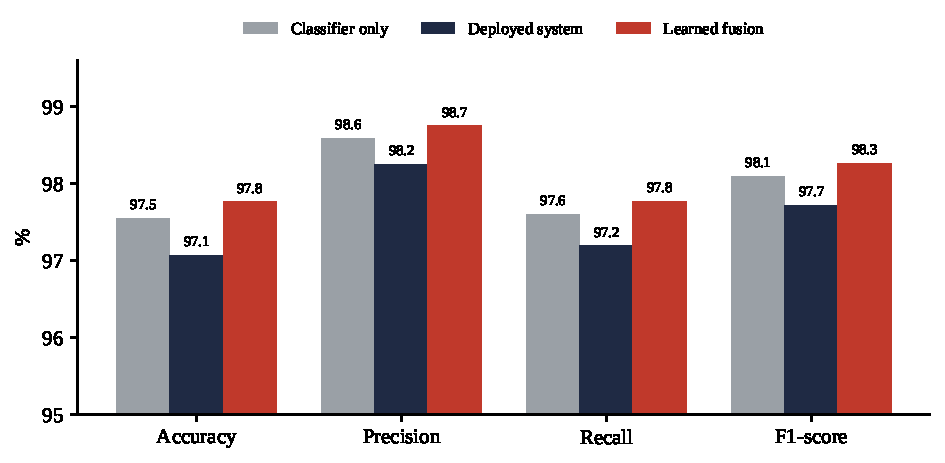
\includegraphics[width=0.62\linewidth]{figures/final_metrics.pdf}
\caption{Accuracy, precision, recall and F1-score on the real test set (vertical axis starts at 95\%)}
\label{fig:final}
\end{figure}

Table~\ref{tab:models} compares the candidate models. Logistic regression with word and character features has the lowest false-alarm rate among the strong models; the SVM's F1 is 0.1 points higher, but it flags 3.9\% of genuine messages.

\begin{table}[H]
\centering
\caption{Candidate models on the real test set (\%)}
\label{tab:models}
\begin{tabular}{|l|l|r|r|r|}
\hline
\textbf{Model} & \textbf{Features} & \textbf{F1} & \textbf{False alarms} & \textbf{Challenge F1} \\
\hline
Naive Bayes & word + char & 95.5 & 6.5 & 86.6 \\
\hline
\textbf{Logistic regression} & \textbf{word + char} & \textbf{98.1} & \textbf{2.6} & 90.2 \\
\hline
Linear SVM & word + char & 98.2 & 3.9 & 92.0 \\
\hline
Random forest & word + char & 97.6 & 3.3 & 73.9 \\
\hline
Logistic regression & word only & 98.0 & 2.7 & 89.9 \\
\hline
Logistic regression & char only & 96.9 & 4.8 & 86.8 \\
\hline
\end{tabular}
\end{table}

Table~\ref{tab:baselines} compares the proposed approach with the usual practice in the literature.

\begin{table}[H]
\centering
\caption{Proposed approach against baseline practice (logistic regression, \%)}
\label{tab:baselines}
\begin{tabular}{|L{5.4cm}|L{4.2cm}|r|r|}
\hline
\textbf{Comparison} & \textbf{Setting} & \textbf{F1} & \textbf{False alarms} \\
\hline
Labels & Report labels (baseline) & 91.2 & 34.0 \\
\cline{2-4}
 & Audited labels (proposed) & 98.1 & 2.6 \\
\hline
Split (real data only) & Random split (baseline) & 98.3 & 0.8 \\
\cline{2-4}
 & Campaign split (proposed) & 97.7 & 1.4 \\
\hline
Training data & Real only & 97.7 & 1.4 \\
\cline{2-4}
 & Real + synthetic (proposed) & 98.1 & 2.6 \\
\hline
\end{tabular}
\end{table}

The label audit has the largest effect: report labels give 99.4\% recall but flag 34.0\% of genuine messages. The random split looks better than the campaign split, but only because 793 of its test messages have a near-duplicate in training; it hides nearly half of the false alarms. Synthetic data costs a little precision on real messages but raises recall on the 2025--26 scam types in the challenge set from 35.6\% to 82.2\%.

\begin{figure}[H]
\centering
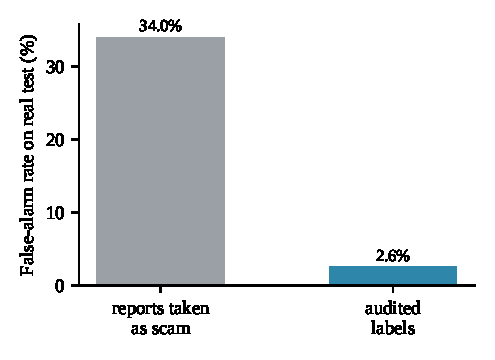
\includegraphics[width=0.5\linewidth]{figures/label_audit.pdf}
\caption{False-alarm rate with report labels and with audited labels}
\label{fig:audit}
\end{figure}

\section{Validation of the proposed approach}
\begin{itemize}
\item \textbf{Confidence intervals.} The deployed system's accuracy lies between 96.3\% and 97.8\%, and its false-alarm rate between 2.0\% and 4.6\% (95\% bootstrap intervals).
\item \textbf{Significance.} Audited labels beat report labels on 210 test messages and lose on 23 (McNemar $p<10^{-30}$). Learned fusion weights are significantly better than the hand-set ones ($p=0.002$) but not better than the classifier alone ($p=0.34$).
\item \textbf{Independent data.} On the 12 advisory messages from 2025--26 the system detects 10 of the 11 scams and passes the one genuine operator notice (F1 95.2\%); the set is too small for a firm conclusion.
\item \textbf{Rules.} On the team's own challenge messages the rules raise F1 from 90.2\% to 95.6\%, but on independent real data they lower it from 98.1\% to 97.7\%. The rules are kept for their phrase-level explanations, not for accuracy.
\end{itemize}

\begin{figure}[H]
\centering
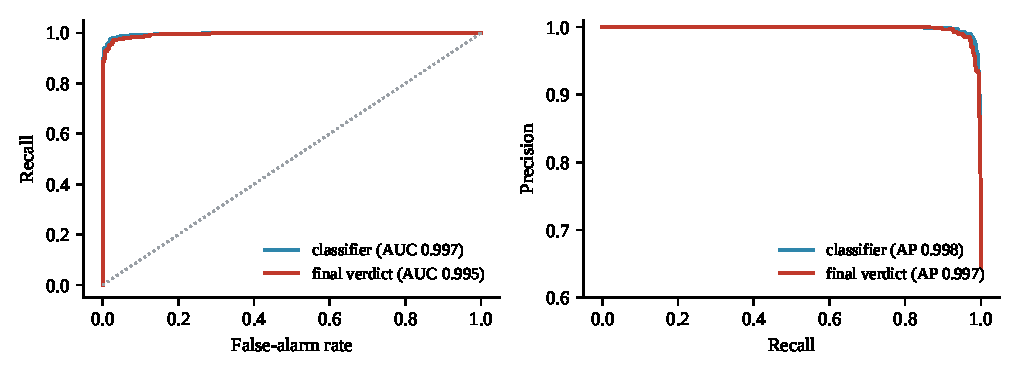
\includegraphics[width=0.9\linewidth]{figures/roc_pr.pdf}
\caption{ROC and precision-recall curves on the real test set}
\label{fig:rocpr}
\end{figure}

\section{Observations}
\begin{figure}[H]
\centering
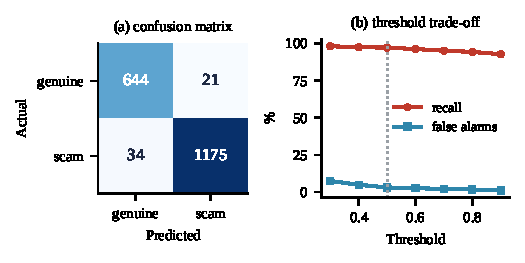
\includegraphics[width=0.68\linewidth]{figures/confusion.pdf}
\caption{(a) Confusion matrix of the deployed system; (b) recall and false-alarm rate by threshold}
\label{fig:conf}
\end{figure}

\begin{itemize}
\item \textbf{Errors.} At the default threshold the system misses 34 scams and flags 21 genuine messages; 15 of the 21 are reported-but-genuine bank messages that ask the user to click a link to finish a KYC or card application.
\item \textbf{Threshold.} A threshold of 0.9 lowers the false-alarm rate to 0.8\% while recall falls to 92.5\%.
\item \textbf{Scam types.} Recall is 97.7\% on banking scams (895 of 916) and 92.3\% on government-themed scams (24 of 26).
\item \textbf{Robustness.} Obfuscating keywords such as KYC, PAN, OTP and SIM in 837 test scams lowered recall from 99.4\% to 98.9\% with word features and to 99.3\% with word and character features.
\item \textbf{Response time and size.} Scoring takes 1.7~ms per message for the classifier and 3.8~ms including the rules; training takes 2.7~s; the model and vectorizer occupy 1.6~MB.
\end{itemize}

\section{Output screens}
Figures~\ref{fig:s1}--\ref{fig:s8} show the deployed application.

\begin{figure}[H]\centering\fbox{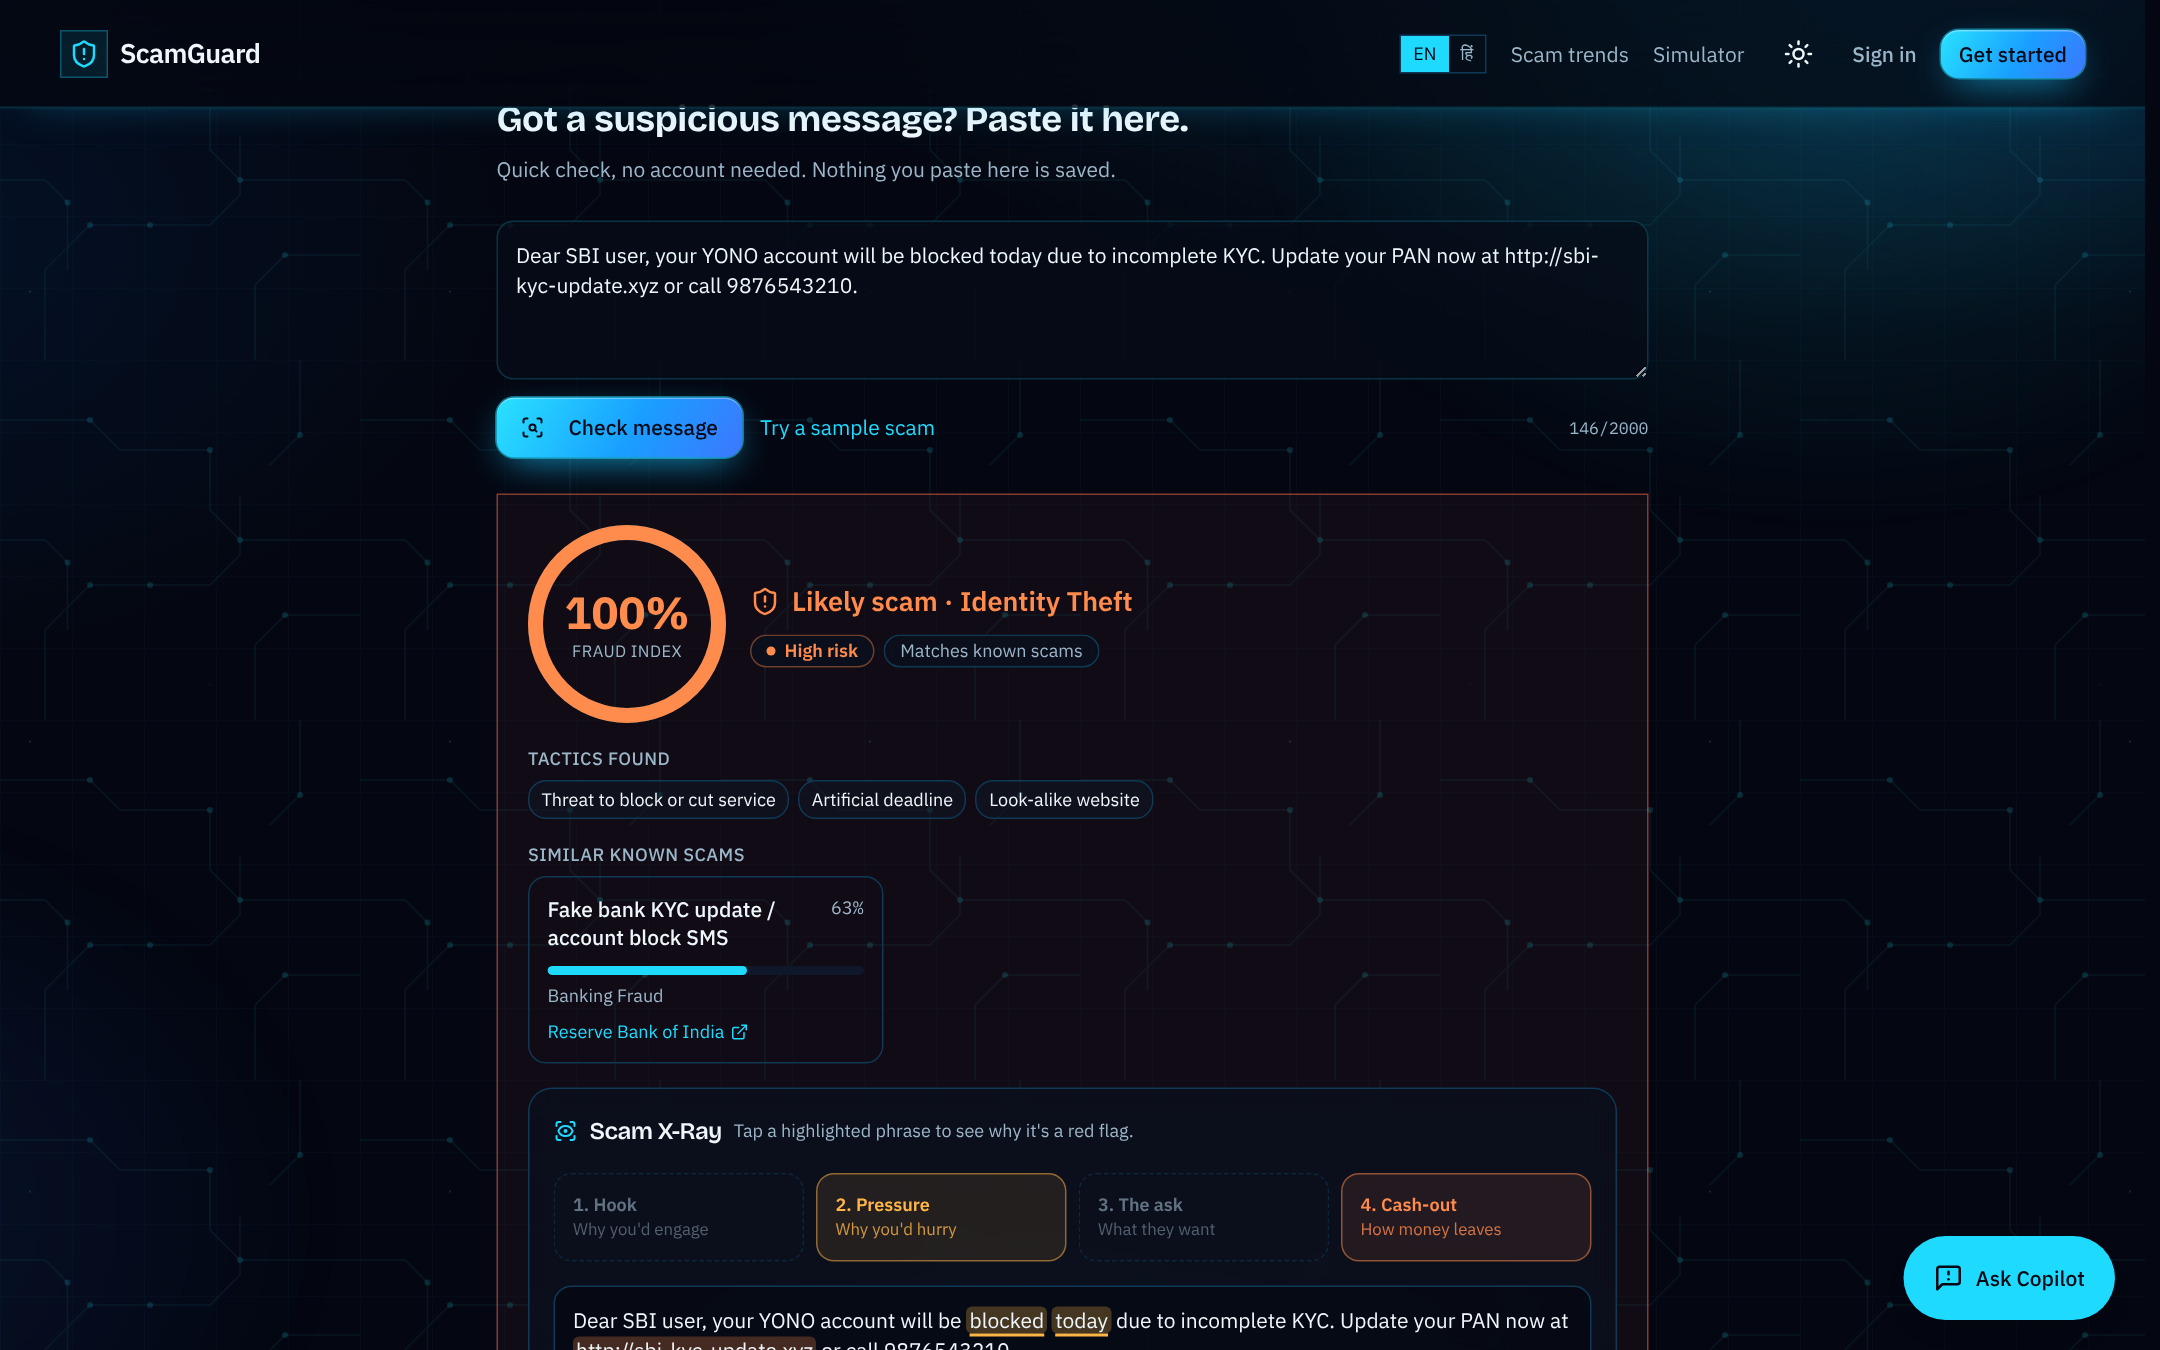
\includegraphics[width=0.78\linewidth]{shots/02_quick_scam.png}}\caption{Quick check of a fake KYC message: verdict, matched tactics and Scam X-Ray}\label{fig:s1}\end{figure}
\begin{figure}[H]\centering\fbox{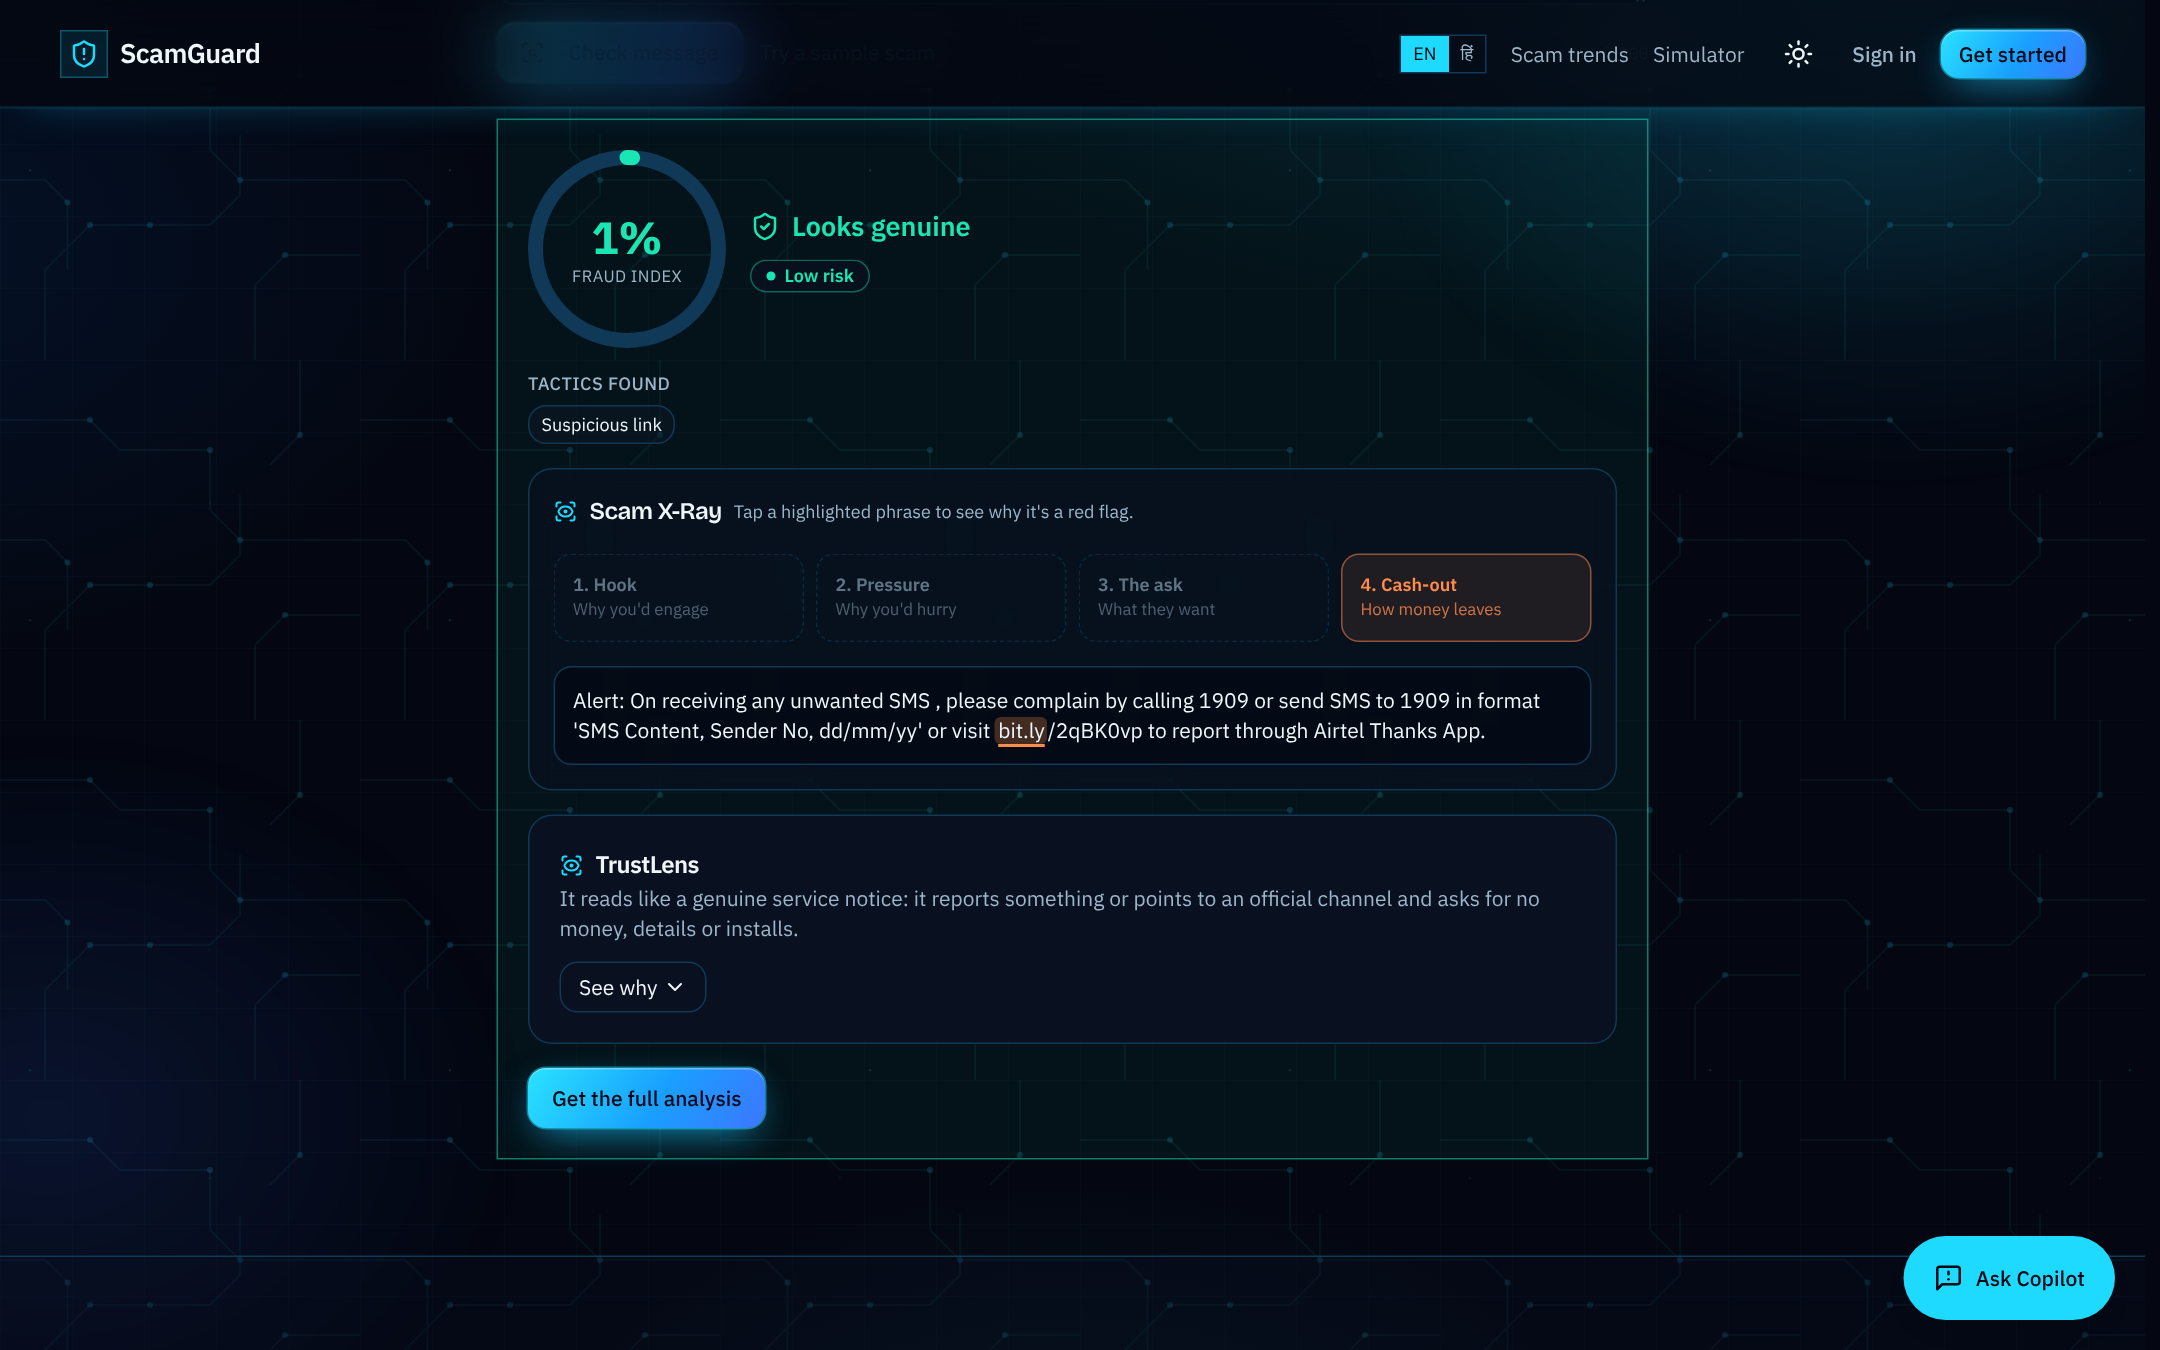
\includegraphics[width=0.78\linewidth]{shots/03_quick_genuine.png}}\caption{Quick check of a genuine operator notice about the 1909 helpline}\end{figure}
\begin{figure}[H]\centering\fbox{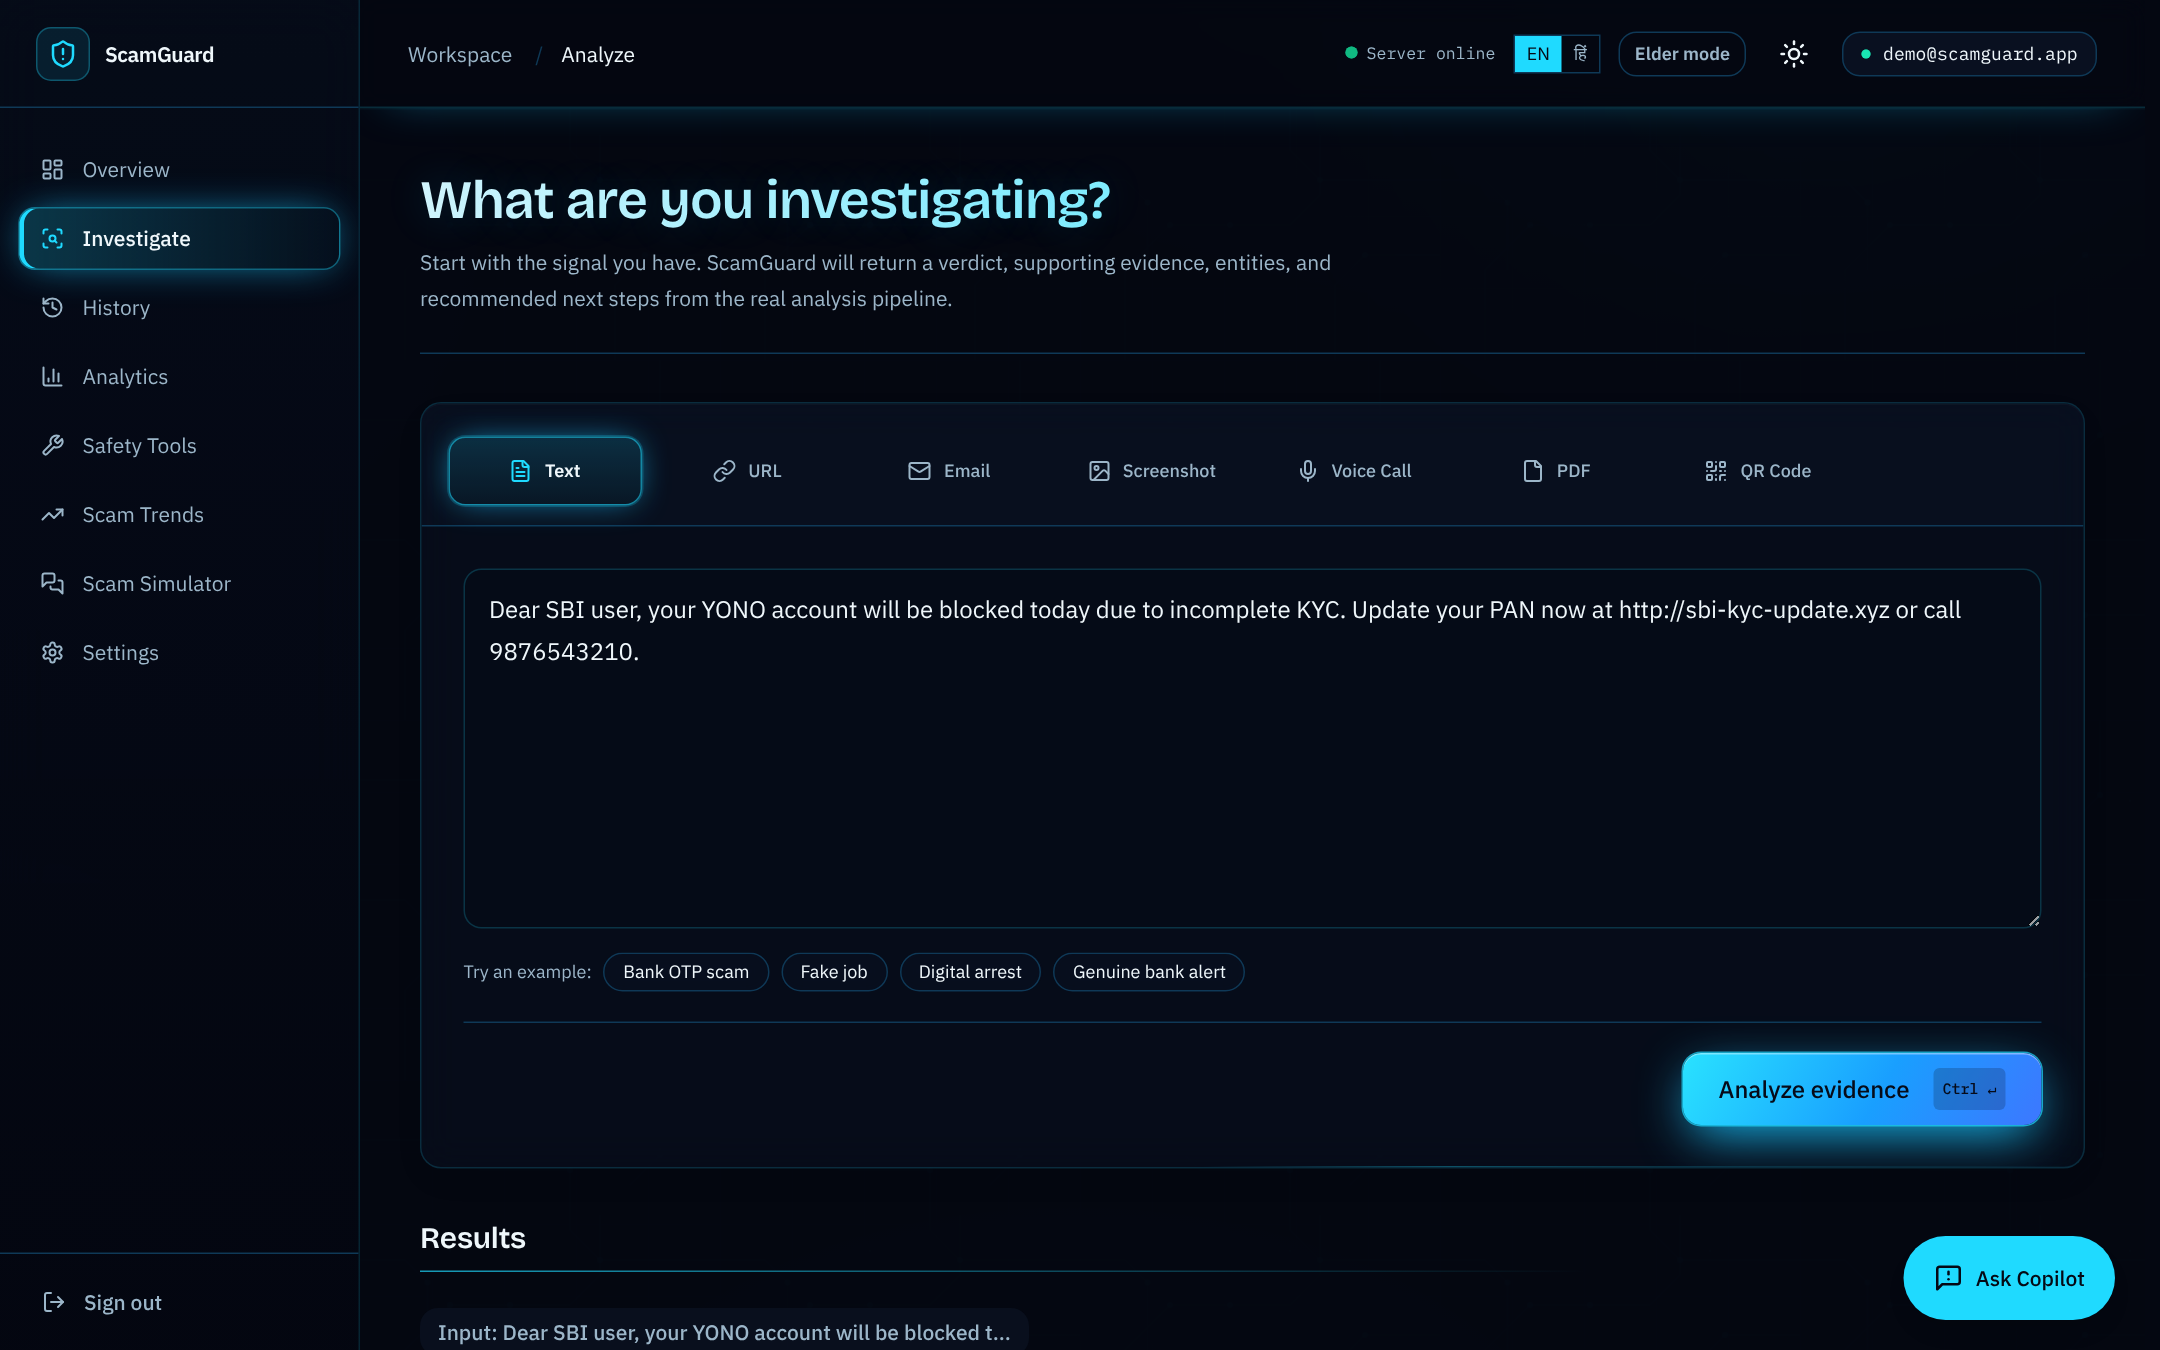
\includegraphics[width=0.78\linewidth]{shots/05_analyze_result.png}}\caption{Full analysis screen for a signed-in user}\end{figure}
\begin{figure}[H]\centering\fbox{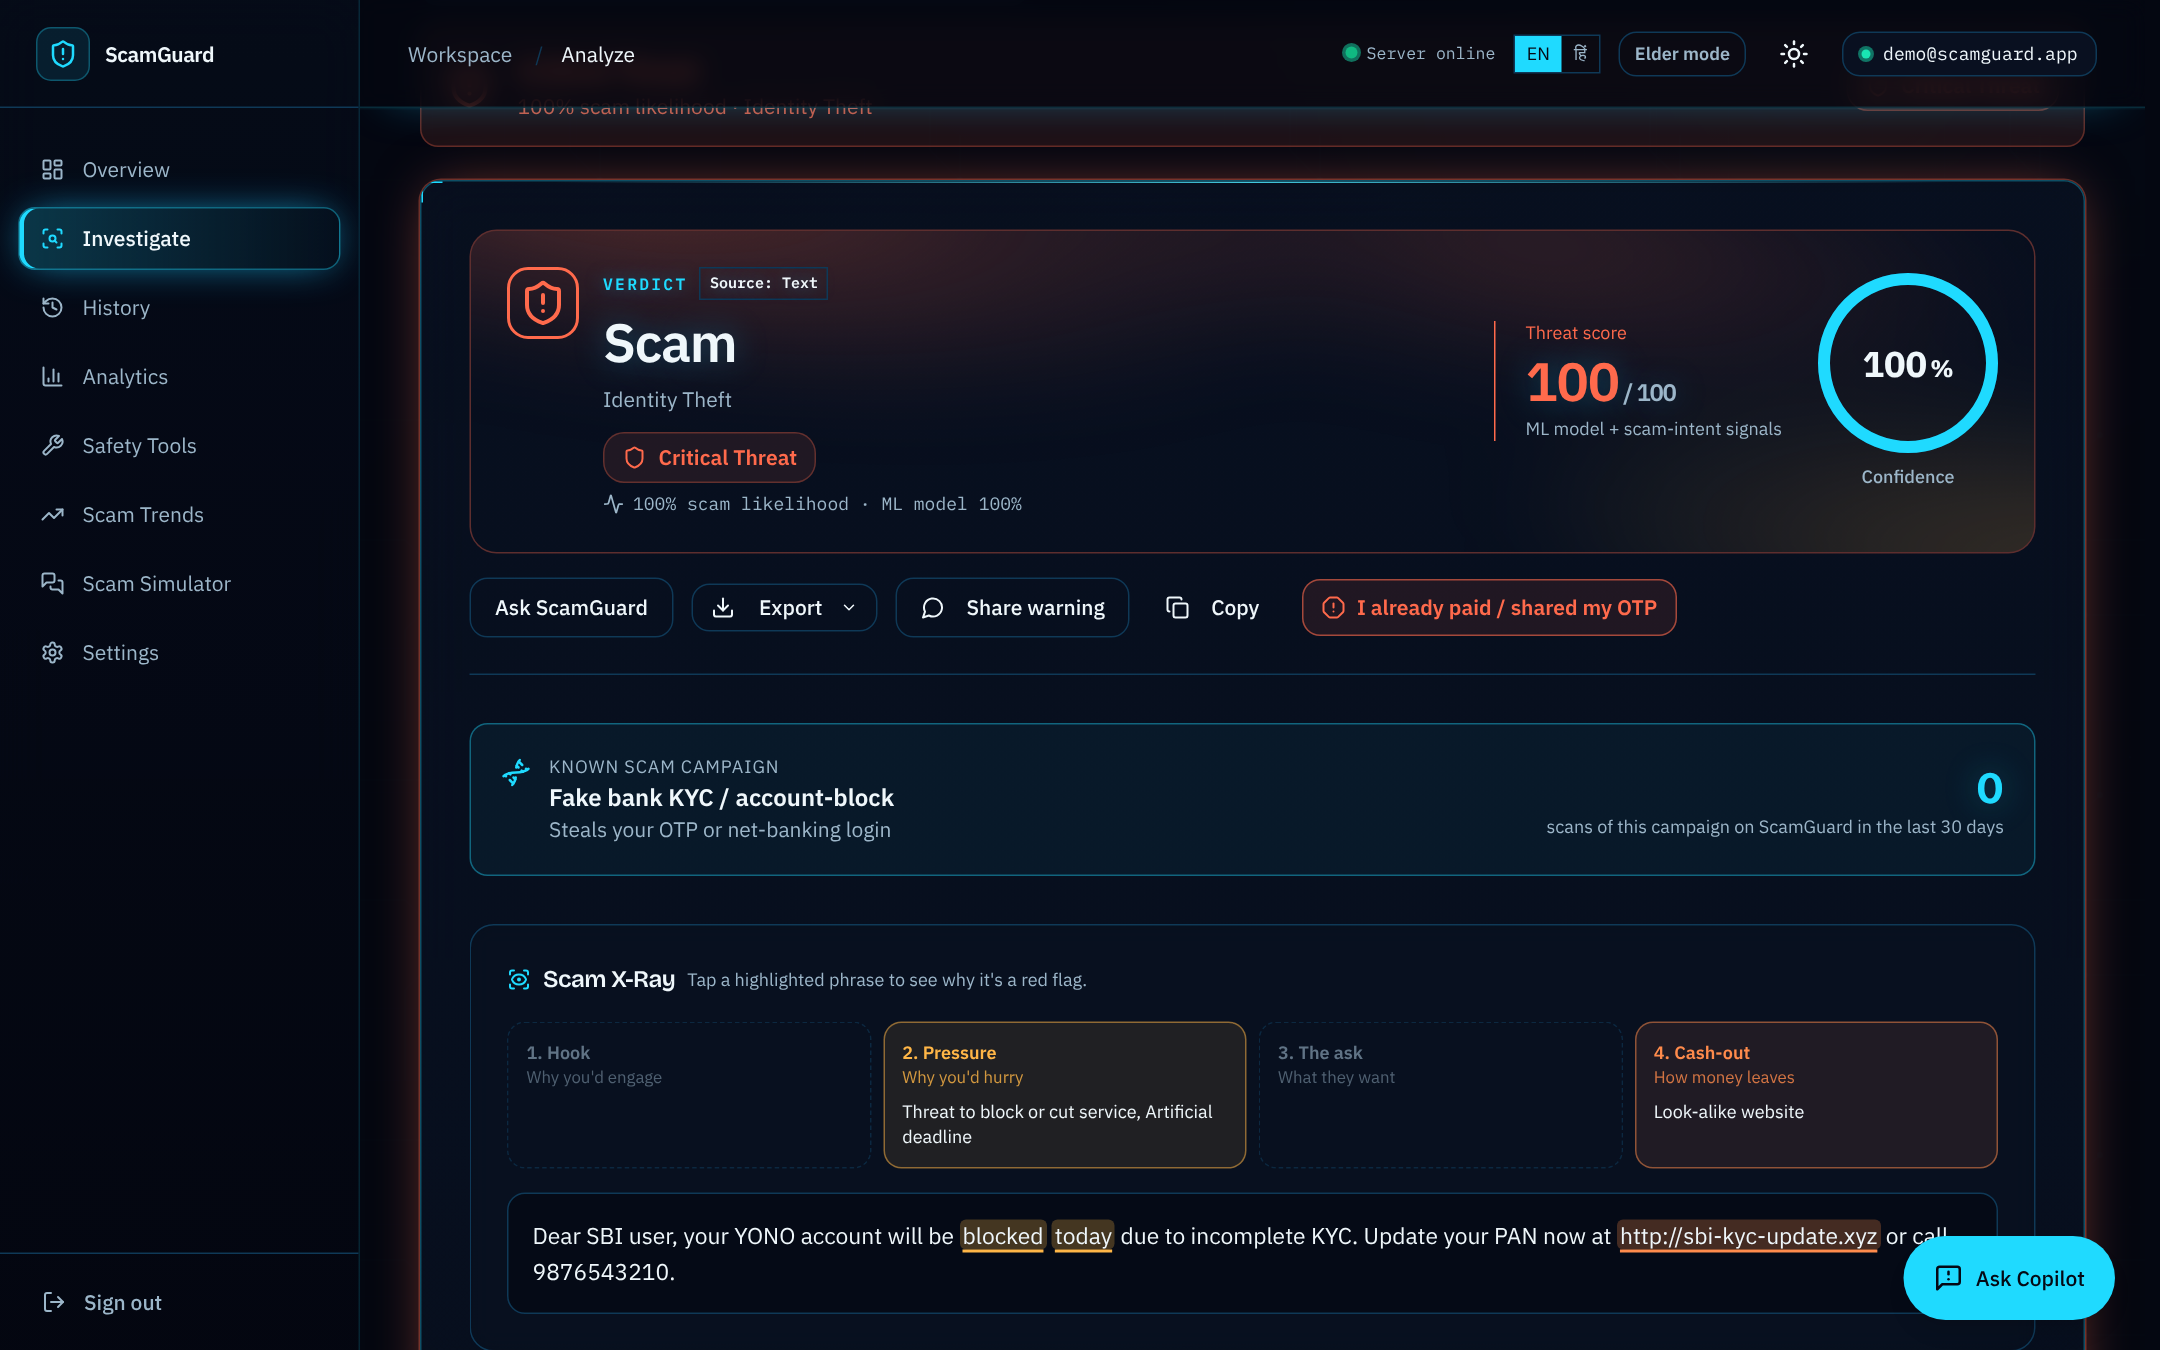
\includegraphics[width=0.78\linewidth]{shots/06_analyze_xray.png}}\caption{Scam X-Ray: each risky phrase placed in the hook, pressure, request and cash-out stages}\end{figure}
\begin{figure}[H]\centering\fbox{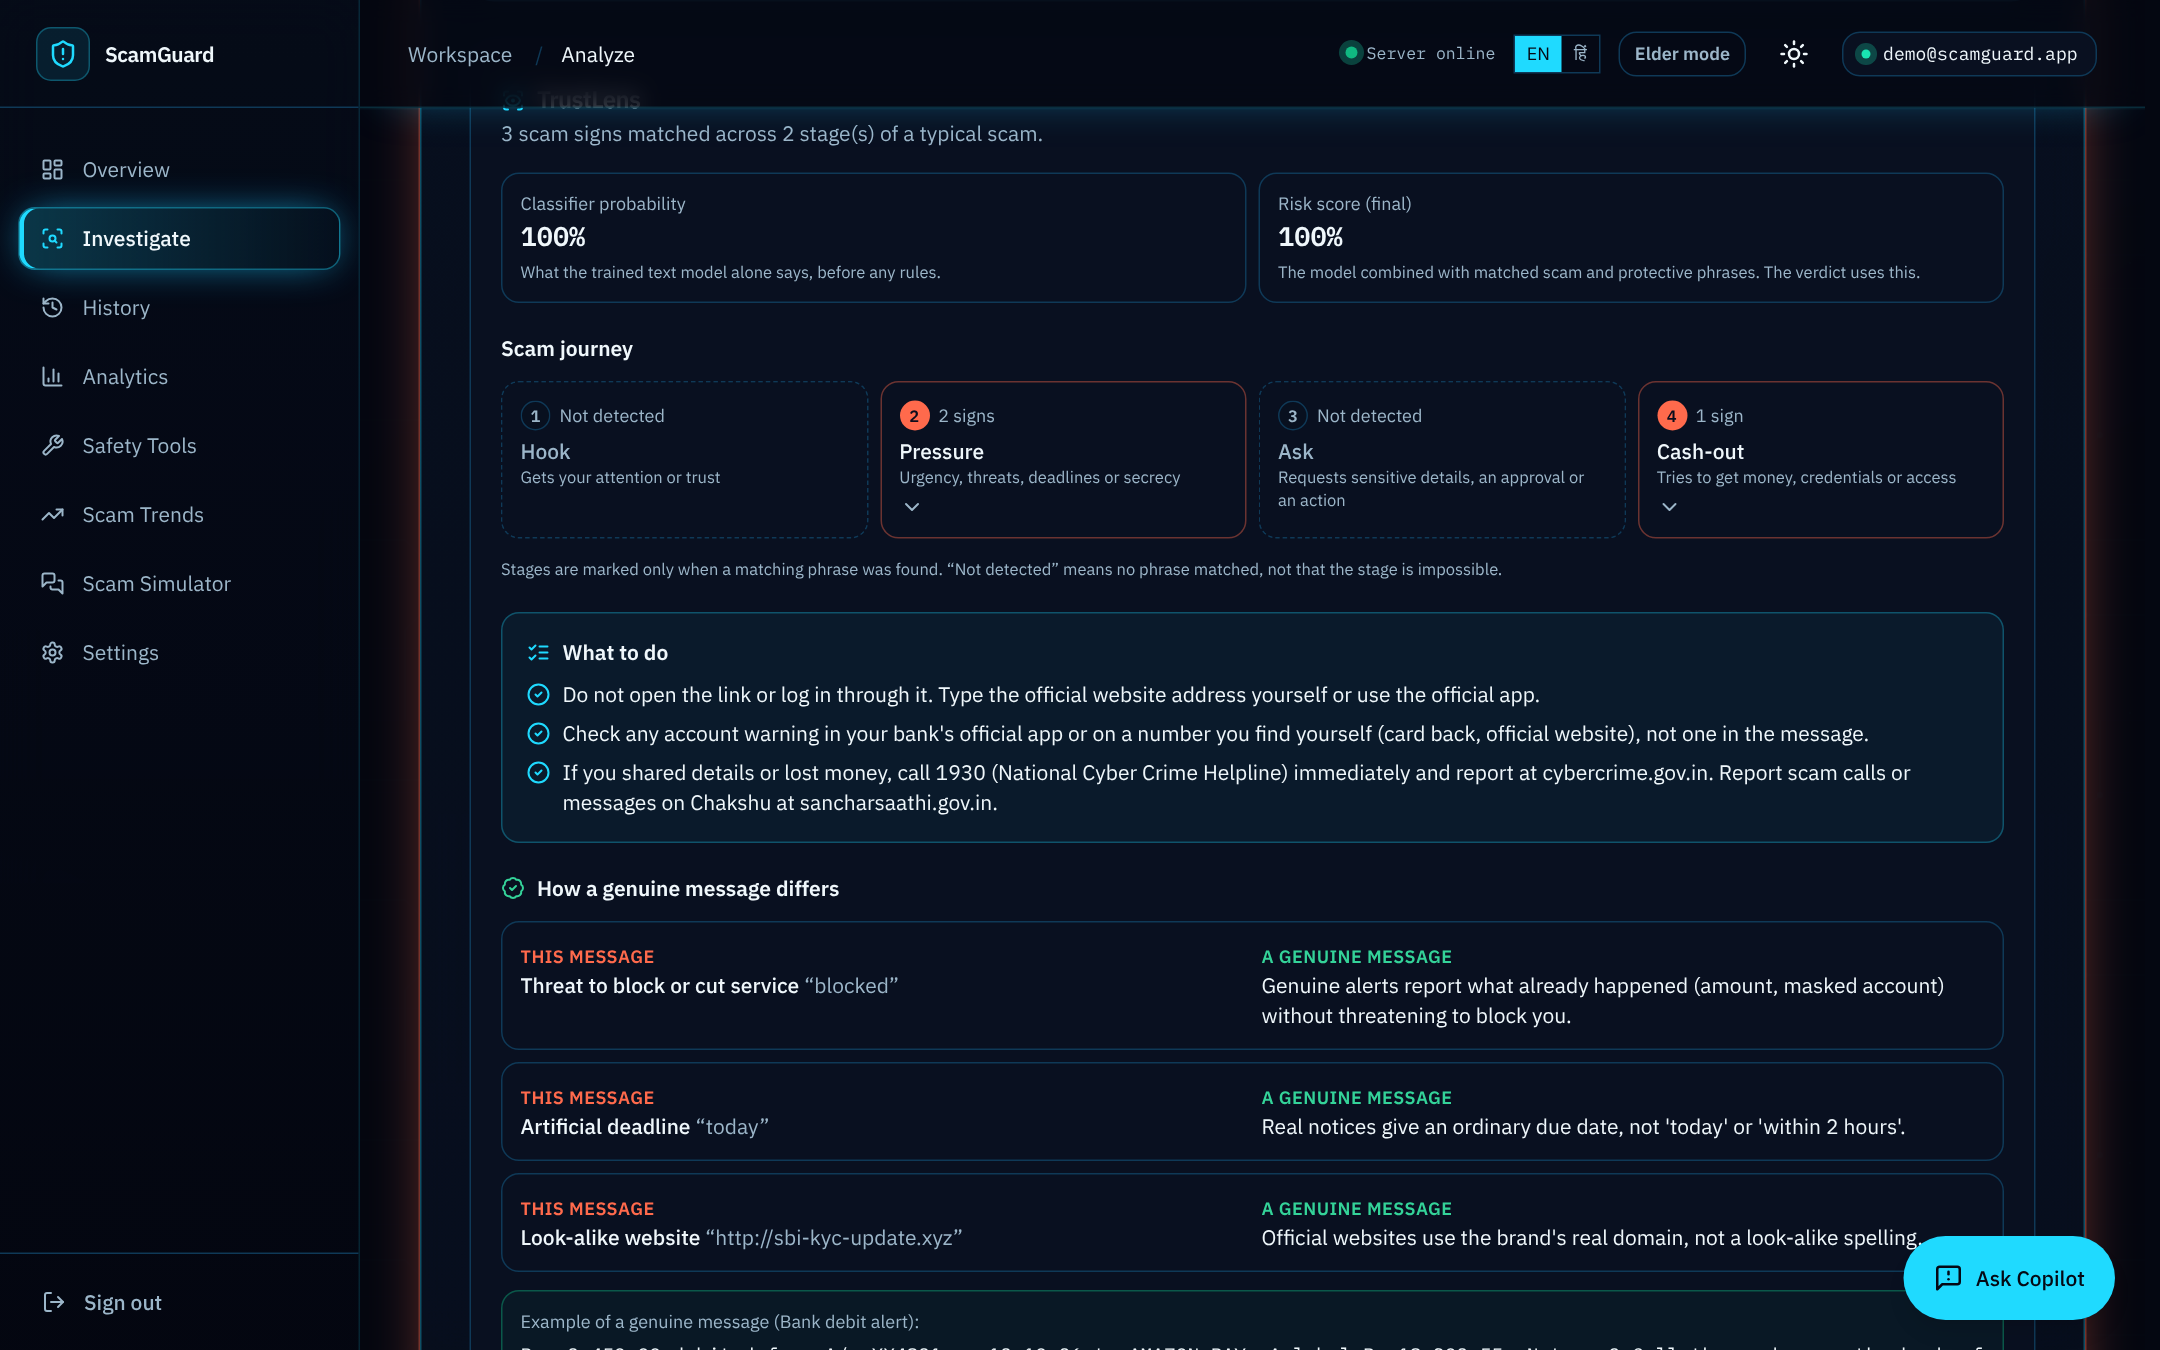
\includegraphics[width=0.78\linewidth]{shots/07_analyze_trustlens.png}}\caption{TrustLens: scam journey, recommended actions and how a genuine message differs}\end{figure}
\begin{figure}[H]\centering\fbox{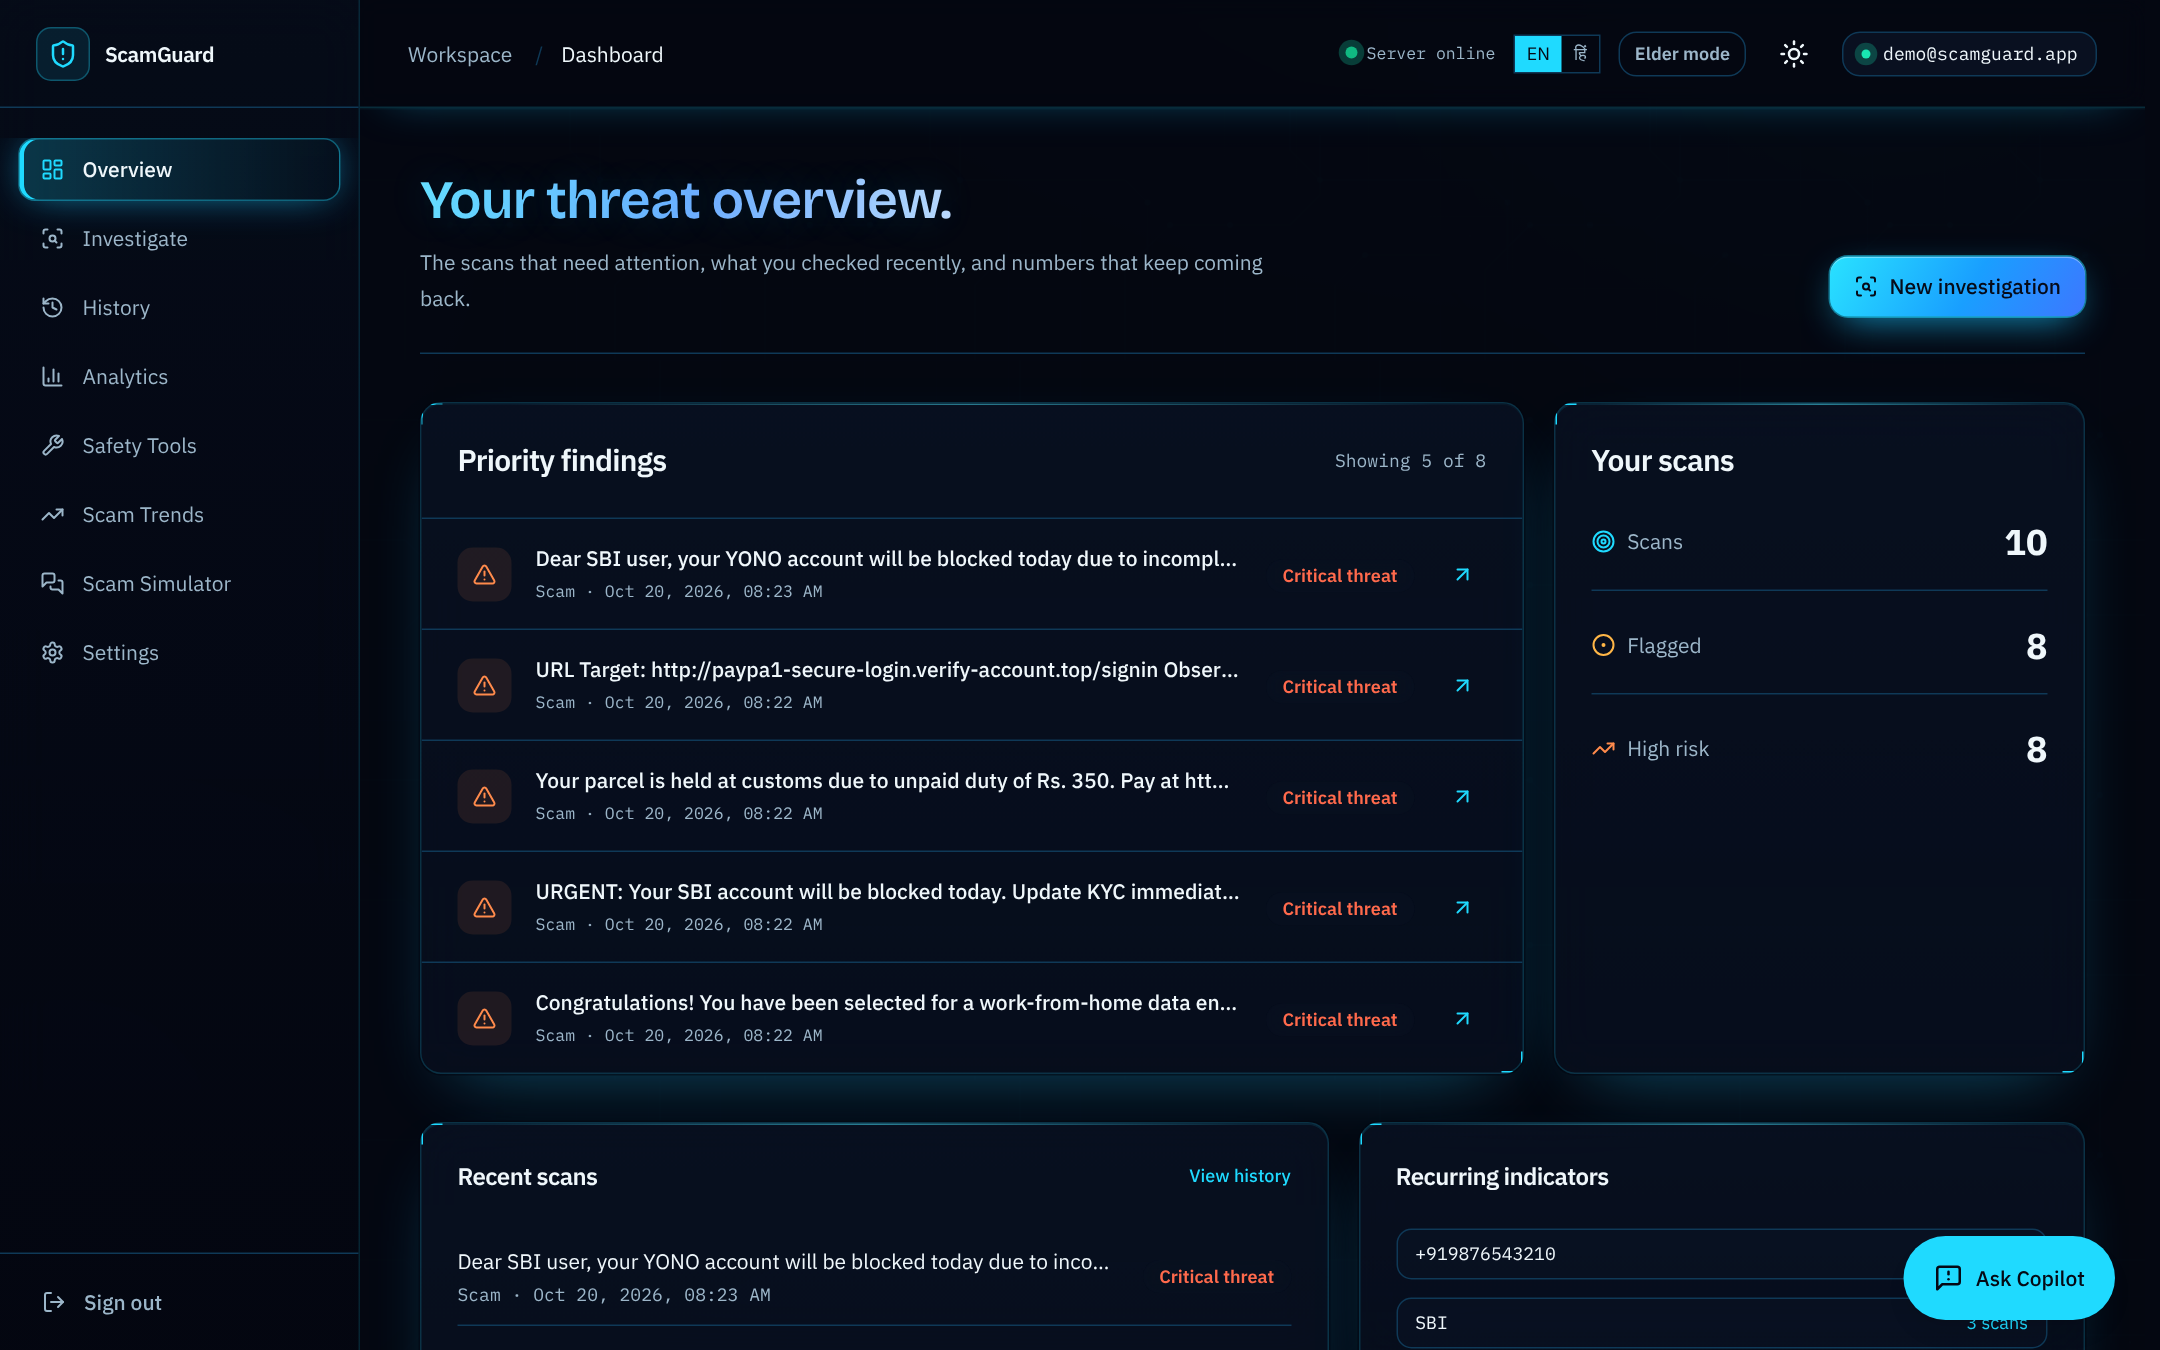
\includegraphics[width=0.78\linewidth]{shots/08_dashboard.png}}\caption{Dashboard with priority findings and recent scans}\end{figure}
\begin{figure}[H]\centering\fbox{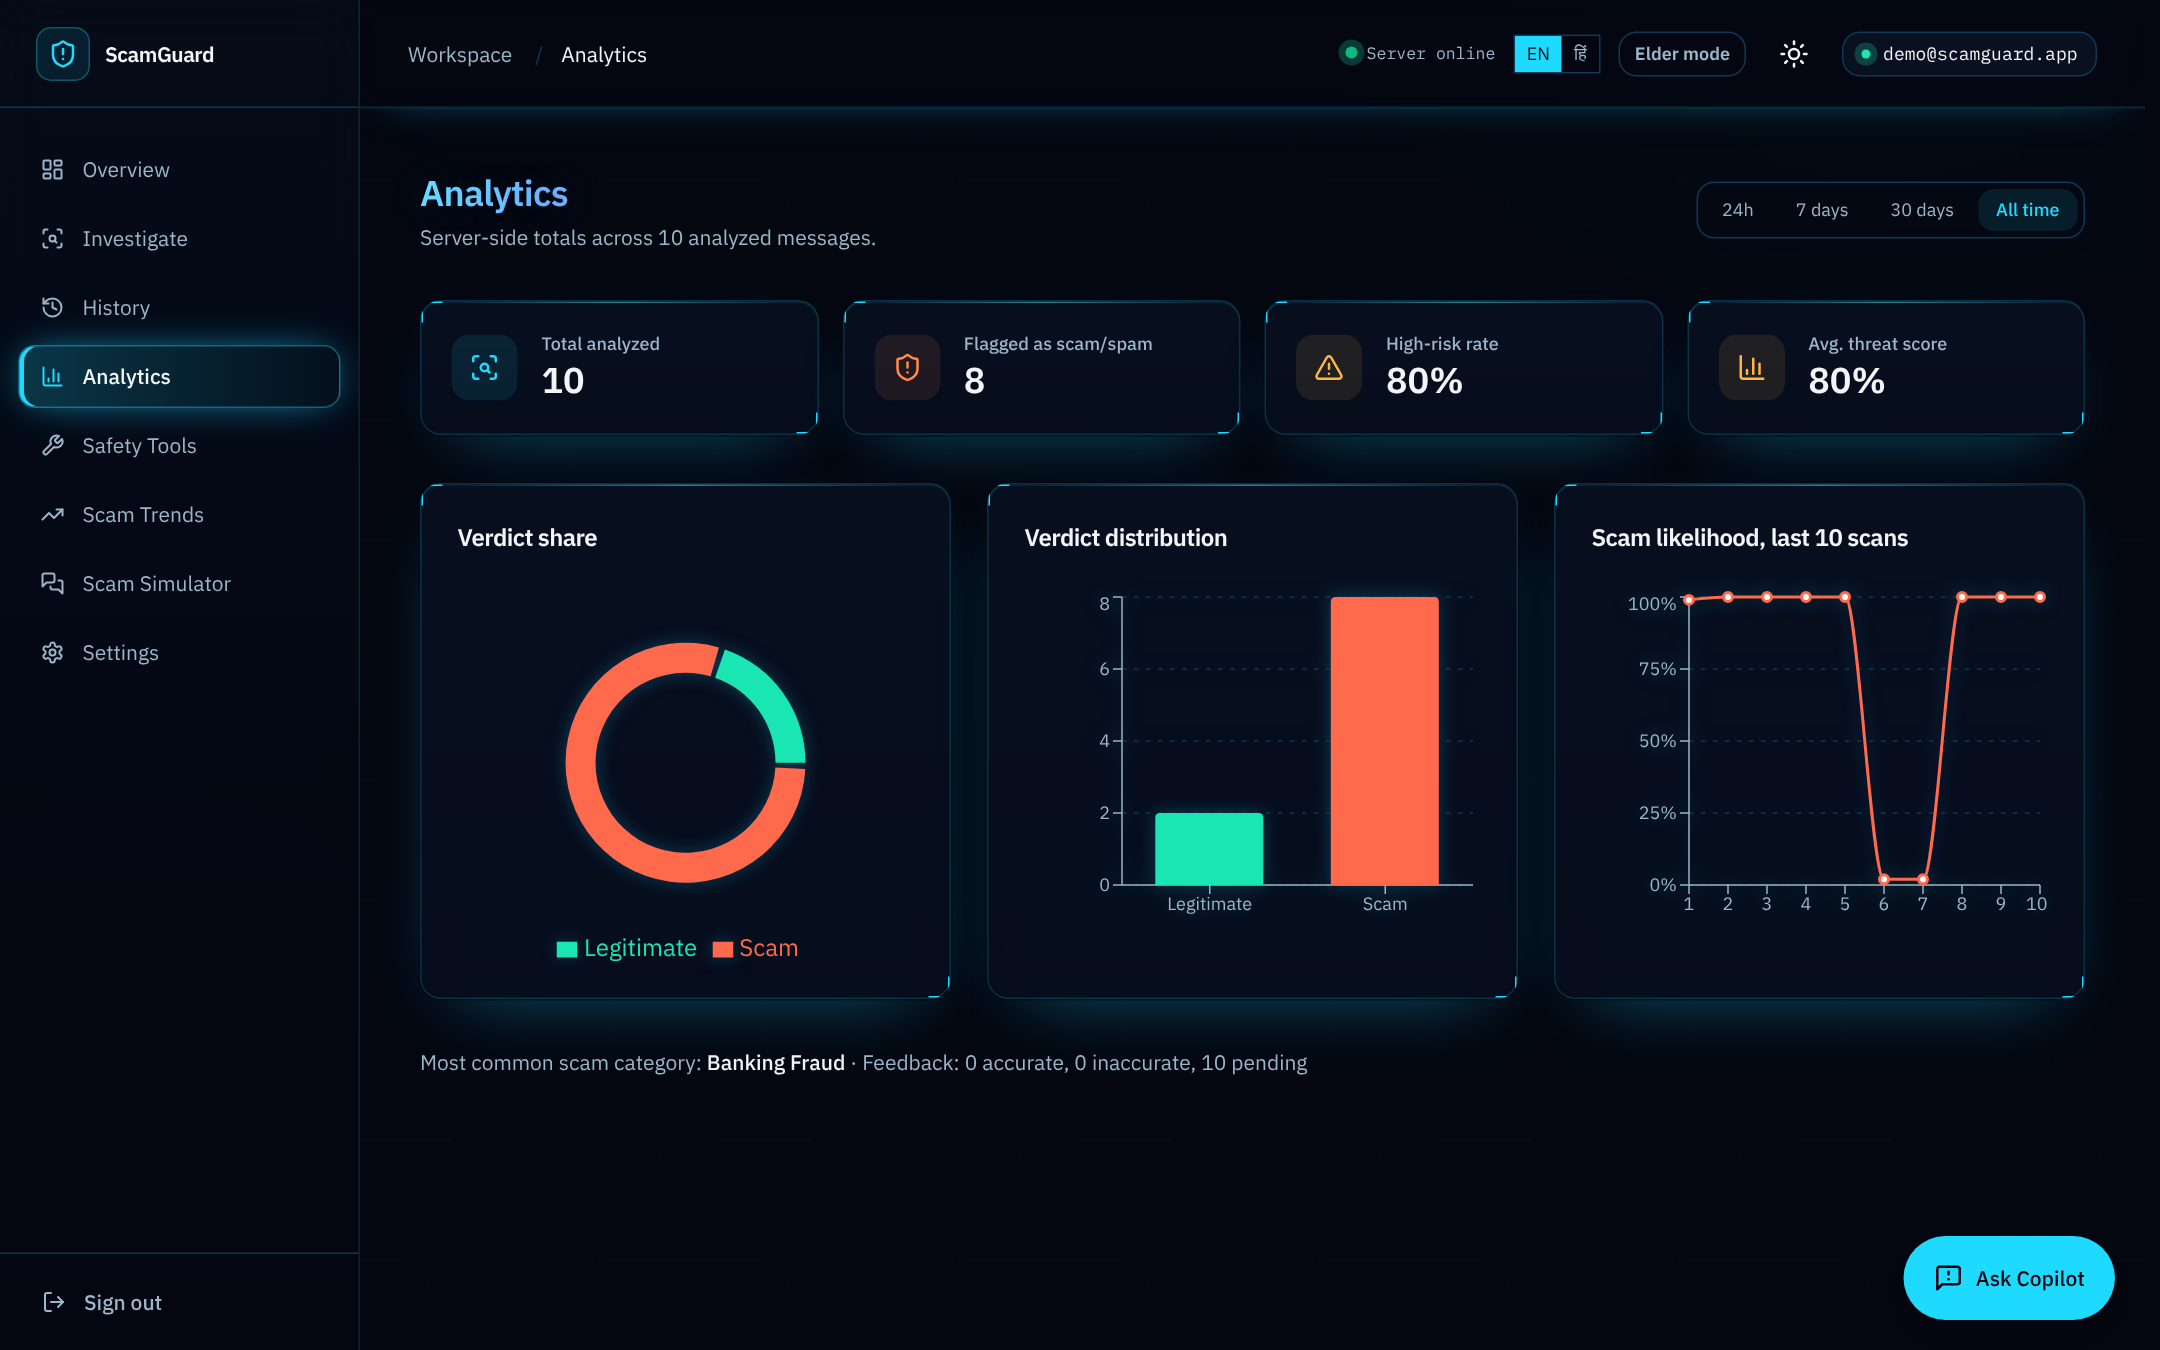
\includegraphics[width=0.78\linewidth]{shots/10_analytics.png}}\caption{Analytics: verdict share and score trend}\end{figure}
\begin{figure}[H]\centering\fbox{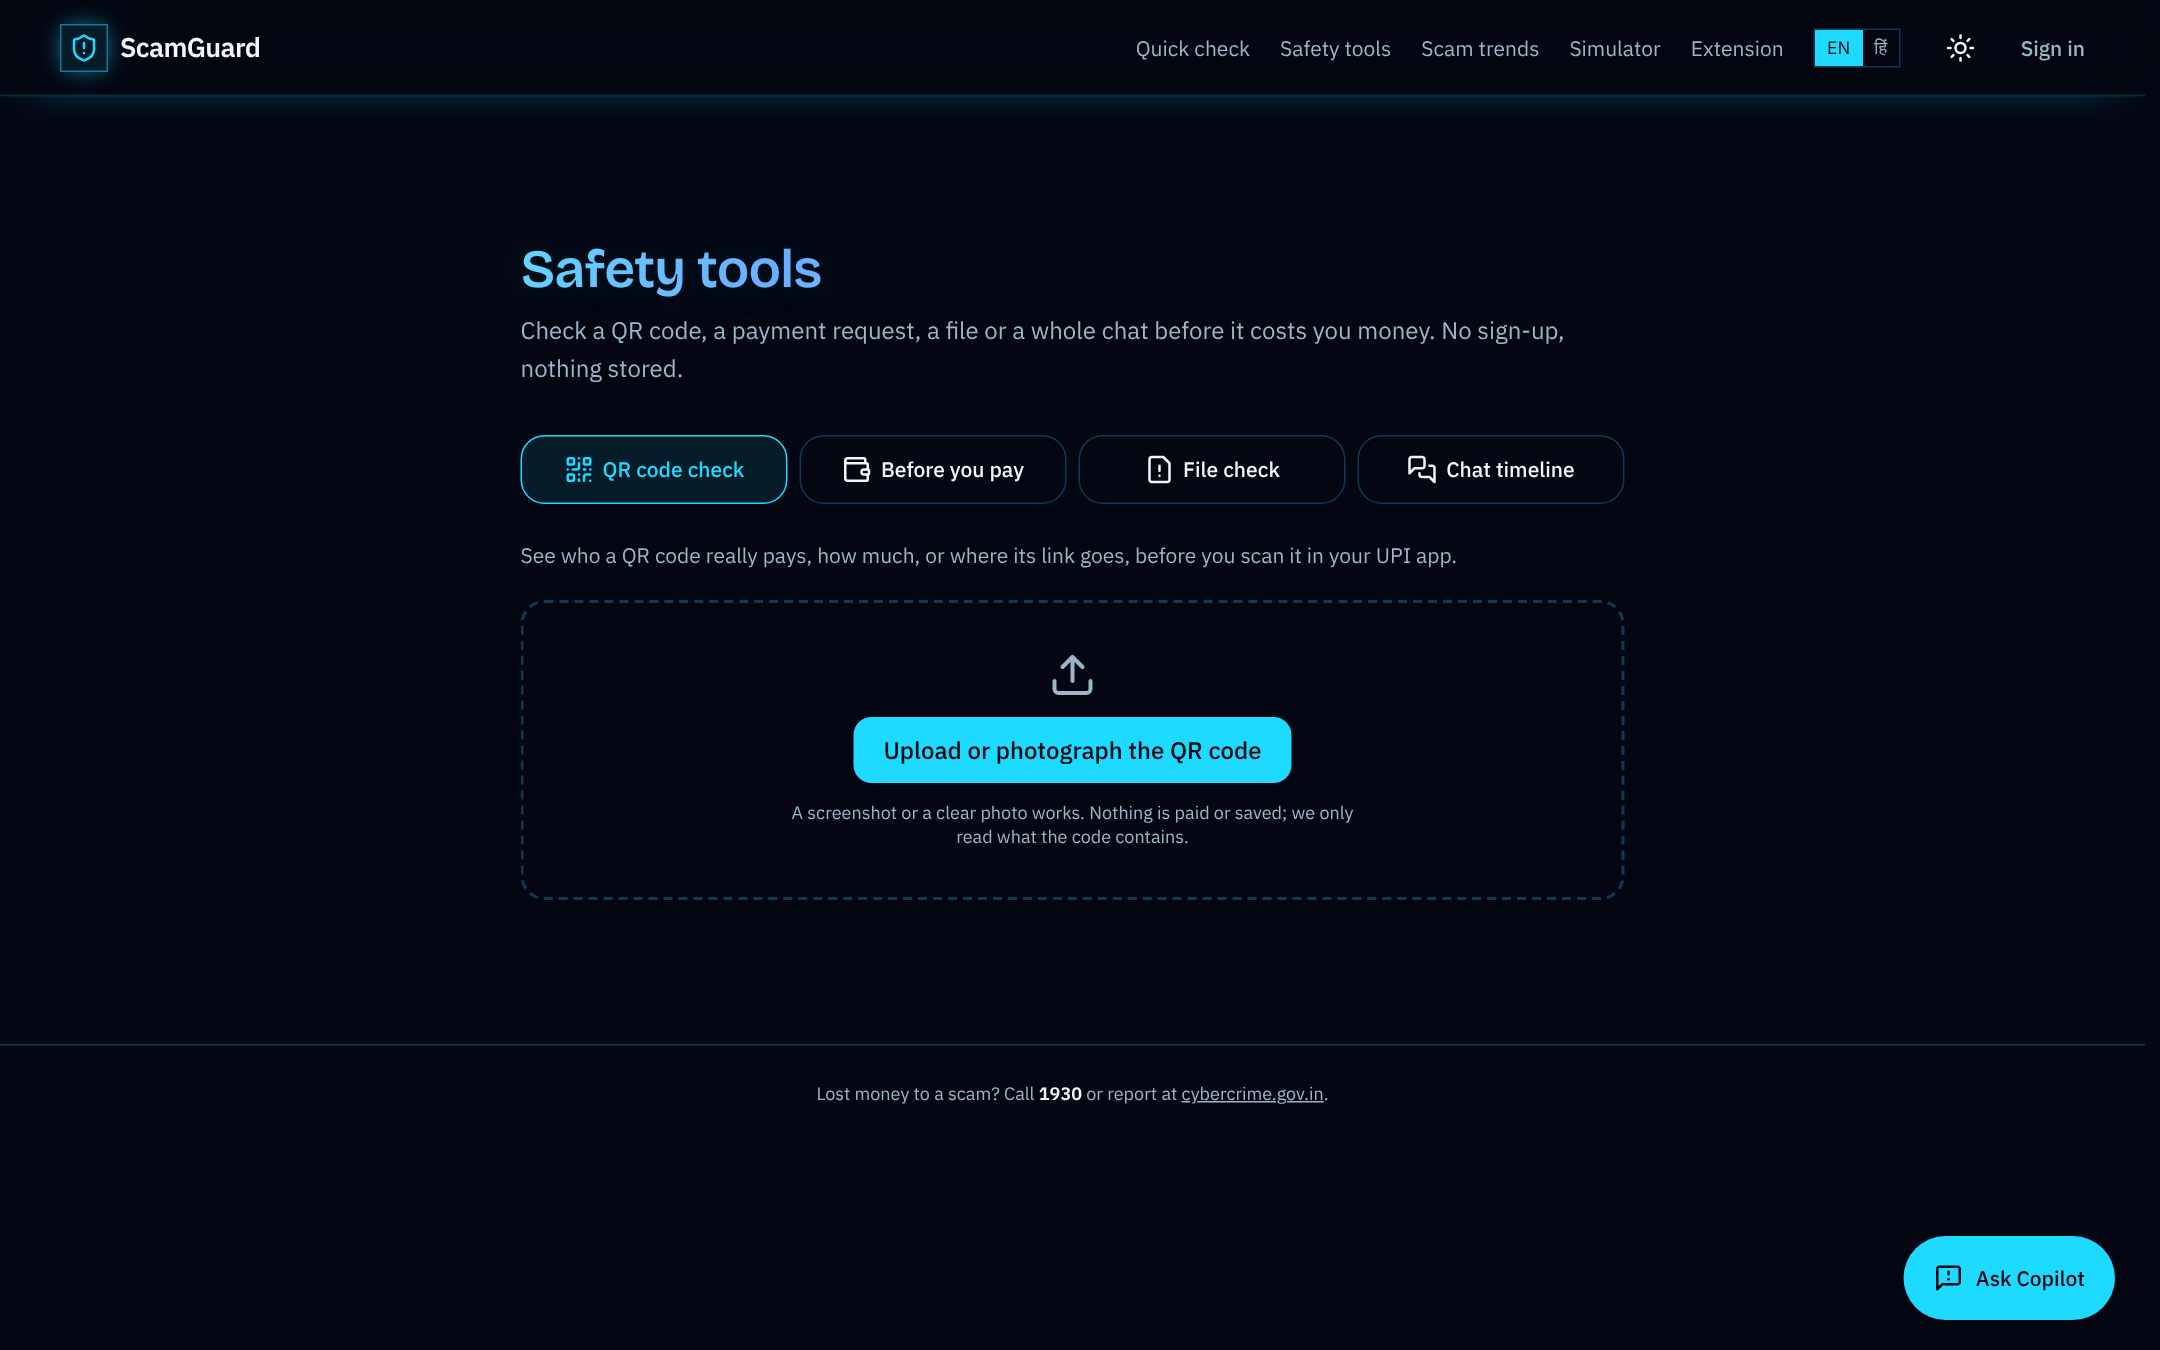
\includegraphics[width=0.78\linewidth]{shots/11_tools.png}}\caption{Safety tools: QR code check, before-you-pay check, file check and chat timeline}\label{fig:s8}\end{figure}

% ======================================================================
\chapter{Conclusion}
\textbf{Performance findings.} On 1,874 real Indian messages from campaigns never seen in training, the deployed ScamGuard system reaches 97.1\% accuracy, 98.2\% precision, 97.2\% recall and a 3.2\% false-alarm rate, with a ROC-AUC of 0.995. It answers in 3.8~ms per message on a two-core server and needs only 1.6~MB for the model.

\textbf{Comparison with the baseline.} The common practice of treating every reported message as a scam flags 34.0\% of genuine messages; the same model trained on audited labels flags 2.6\%. A random split hides nearly half of the false alarms that a campaign-aware split reveals. Hand-written rules look strong on the developers' own messages but do not improve accuracy on independent data.

\textbf{Contribution to the research gap.} ScamGuard-IN-2026 provides what the literature lacked: an Indian scam-versus-genuine SMS dataset with a verified genuine class, an audit record for every reported-message group and a split that keeps each scam campaign on one side. The detector evaluated on it is deployed as an explainable client--server application.

\textbf{Limitations.} The 2025--26 scam types are represented in testing by only 12 advisory messages. One annotator made the manual decisions. Synthetic training data shares authors with the rules. Languages other than English and Hindi are not covered, and only simple obfuscation was tested.

\textbf{Future work.} Collect a larger real 2026 test set from team members, add a second annotator, extend to Kannada, Tamil and Telugu, test against paraphrased and adaptive scams, compare with small transformer models under the same split, and offer an Android share-to-check feature.

\section{Mapping to course outcomes}
Table~\ref{tab:co} relates the work to the course outcomes of Major Project Phase-2 (23CS7PWPP2), and Table~\ref{tab:copo} gives the CO--PO--PSO mapping of the course.

\begin{table}[H]
\centering
\caption{Course outcomes and where they are addressed}
\label{tab:co}
\begin{tabular}{|c|L{6.6cm}|L{6.1cm}|}
\hline
\textbf{CO} & \textbf{Course outcome} & \textbf{Addressed in this work} \\
\hline
CO1 & Apply software engineering principles in planning, design and requirements within legal, societal and environmental constraints & Chapters 6--7: problem statement, architecture, sub-systems; licensed data and masking of personal data \\
\hline
CO2 & Apply mathematics, science and engineering to implement the project and draw conclusions with integrity & Chapter 7: mathematical model; Chapter 9: reported results with confidence intervals \\
\hline
CO3 & Monitor and manage schedules, resources and work assignments & Section 7.9: timeline, resources and cost \\
\hline
CO4 & Test and defend the performance of the implemented project & Section 7.8 and Chapters 8--9: tests, metrics and validation \\
\hline
CO5 & Work individually and as a team & Shared work on data, model, back end and front end \\
\hline
CO6 & Communicate, present and prepare technical documents & This report, the research paper and the presentation \\
\hline
\end{tabular}
\end{table}

\begin{table}[H]
\centering
\caption{CO--PO--PSO mapping of Major Project Phase-2}
\label{tab:copo}
\footnotesize
\setlength{\tabcolsep}{2.6pt}
\begin{tabular}{|c|c|c|c|c|c|c|c|c|c|c|c|c|c|c|c|}
\hline
 & \textbf{PO1} & \textbf{PO2} & \textbf{PO3} & \textbf{PO4} & \textbf{PO5} & \textbf{PO6} & \textbf{PO7} & \textbf{PO8} & \textbf{PO9} & \textbf{PO10} & \textbf{PO11} & \textbf{PO12} & \textbf{PSO1} & \textbf{PSO2} & \textbf{PSO3} \\
\hline
CO1 & & 2 & 2 & & & 2 & 2 & & & & & 2 & 2 & & \\
\hline
CO2 & 3 & & & 3 & 3 & & & 3 & & & & & & 3 & 3 \\
\hline
CO3 & & & & & & & & & & & 3 & & & & \\
\hline
CO4 & & & & & & & 1 & & & & & & & & 1 \\
\hline
CO5 & & & & & & & & & 1 & & & 1 & & & \\
\hline
CO6 & & & & & & & & & & 2 & & 2 & & & \\
\hline
\end{tabular}
\end{table}


% ======================================================================
\clearpage
\renewcommand{\bibname}{References}
\begin{thebibliography}{99}
\addcontentsline{toc}{chapter}{\protect\numberline{11}References}
\bibitem{agarwal2025fishing} S. Agarwal, A. Papasavva, G. Suarez-Tangil, and M. Vasek, ``Fishing for smishing: Understanding SMS phishing infrastructure and strategies by mining public user reports,'' in \textit{Proc. ACM Internet Measurement Conference (IMC '25)}, Madison, WI, USA, 2025, doi: 10.1145/3730567.3764431.
\bibitem{agarwal2026overview} S. Agarwal, G. Suarez-Tangil, and M. Vasek, ``An overview of 7726 user reports: Uncovering SMS scams and scammer strategies,'' in \textit{Proc. Network and Distributed System Security Symposium (NDSS)}, San Diego, CA, USA, 2026.
\bibitem{pritom2026sms} M. M. A. Pritom, S. M. Sanjari, M. Mia, A. M. Shibli, S. M. M. Hossain, M. Ismail, and S. Xu, ``Short message service (SMS) phishing attacks and defenses: A systematic review,'' arXiv:2604.11429, 2026.
\bibitem{almeida2011contributions} T. A. Almeida, J. M. G\'omez Hidalgo, and A. Yamakami, ``Contributions to the study of SMS spam filtering: New collection and results,'' in \textit{Proc. 11th ACM Symposium on Document Engineering}, Mountain View, CA, USA, 2011, pp. 259--262.
\bibitem{almeida2013towards} T. A. Almeida, J. M. G\'omez Hidalgo, and T. P. Silva, ``Towards SMS spam filtering: Results under a new dataset,'' \textit{International Journal of Information Security Science}, vol. 2, no. 1, pp. 1--18, 2013.
\bibitem{roy2020deep} P. K. Roy, J. P. Singh, and S. Banerjee, ``Deep learning to filter SMS spam,'' \textit{Future Generation Computer Systems}, vol. 102, pp. 524--533, 2020.
\bibitem{mishra2020smishing} S. Mishra and D. Soni, ``Smishing Detector: A security model to detect smishing through SMS content analysis and URL behavior analysis,'' \textit{Future Generation Computer Systems}, 2020.
\bibitem{sonowal2018smidca} G. Sonowal and K. S. Kuppusamy, ``SmiDCA: An anti-smishing model with machine learning approach,'' \textit{The Computer Journal}, vol. 61, no. 8, pp. 1143--1157, 2018, doi: 10.1093/comjnl/bxy039.
\bibitem{goel2024ml} D. Goel, H. Ahmad, A. K. Jain, and N. K. Goel, ``Machine learning driven smishing detection framework for mobile security,'' arXiv:2412.09641, 2024.
\bibitem{timko2024smishing} D. Timko and M. L. Rahman, ``Smishing Dataset I: Phishing SMS dataset from Smishtank.com,'' in \textit{Proc. 14th ACM Conference on Data and Application Security and Privacy (CODASPY '24)}, Porto, Portugal, 2024, doi: 10.1145/3626232.3653282.
\bibitem{ali2025moz} F. D. M. A. Ali, S. M. Saide, R. Sousa-Silva, and H. Lopes Cardoso, ``MOZ-Smishing: A benchmark dataset for detecting mobile money frauds,'' in \textit{Proc. 6th Workshop on African Natural Language Processing}, Vienna, Austria, 2025, pp. 158--166, doi: 10.18653/v1/2025.africanlp-1.23.
\bibitem{labonne2023spamt5} M. Labonne and S. Moran, ``Spam-T5: Benchmarking large language models for few-shot email spam detection,'' arXiv:2304.01238, 2023.
\bibitem{ahmadi2025llm} M. Ahmadi, M. Khajavi, A. Varmaghani, A. Ala, K. Danesh, and D. Javaheri, ``Leveraging large language models for cybersecurity: Enhancing SMS spam detection with robust and context-aware text classification,'' arXiv:2502.11014, 2025.
\bibitem{northcutt2021confident} C. Northcutt, L. Jiang, and I. Chuang, ``Confident learning: Estimating uncertainty in dataset labels,'' \textit{Journal of Artificial Intelligence Research}, vol. 70, pp. 1373--1411, 2021, doi: 10.1613/jair.1.12125.
\bibitem{lee2022dedup} K. Lee, D. Ippolito, A. Nystrom, C. Zhang, D. Eck, C. Callison-Burch, and N. Carlini, ``Deduplicating training data makes language models better,'' in \textit{Proc. 60th Annual Meeting of the ACL}, Dublin, Ireland, 2022, pp. 8424--8445, doi: 10.18653/v1/2022.acl-long.577.
\bibitem{kapoor2023leakage} S. Kapoor and A. Narayanan, ``Leakage and the reproducibility crisis in machine-learning-based science,'' \textit{Patterns}, 2023, doi: 10.1016/j.patter.2023.100804.
\bibitem{broder1997resemblance} A. Z. Broder, ``On the resemblance and containment of documents,'' in \textit{Proc. Compression and Complexity of SEQUENCES 1997}, Positano, Italy, 1997, doi: 10.1109/SEQUEN.1997.666900.
\bibitem{salton1988term} G. Salton and C. Buckley, ``Term-weighting approaches in automatic text retrieval,'' \textit{Information Processing \& Management}, vol. 24, no. 5, pp. 513--523, 1988, doi: 10.1016/0306-4573(88)90021-0.
\bibitem{pedregosa2011scikit} F. Pedregosa \textit{et al.}, ``Scikit-learn: Machine learning in Python,'' \textit{Journal of Machine Learning Research}, vol. 12, pp. 2825--2830, 2011.
\bibitem{fastapi} S. Ram\'irez, ``FastAPI documentation,'' 2026. [Online]. Available: https://fastapi.tiangolo.com
\bibitem{nextjs} Vercel, ``Next.js documentation,'' 2026. [Online]. Available: https://nextjs.org/docs
\end{thebibliography}

\end{document}
